\documentclass{beamer}
\usetheme{default}
\definecolor{LiUblue}{RGB}{0,185,231}
\usecolortheme[named=LiUblue]{structure}
%\beamerdefaultoverlayspecification{<+->}
\title{Quantifying nitrogen oxides and ammonia via frequency modulation in gas sensors}
\subtitle{Master Thesis defense seminar}
\author{Marcos F Mourão}
\date{June $1^{st}$ 2021}
 \
\usepackage{booktabs}
 \usepackage{chemformula}
 \usepackage{url}
 \usepackage{chemformula}
 \usepackage{xspace}
 \usepackage{fixltx2e}
 \usepackage{subscript}
 \usepackage{subcaption}
 \usepackage{graphicx}
  \geometry{papersize={12.8cm,10cm}}
 \newcommand{\nox}{\texorpdfstring{NO\textsubscript{x}}{NOx}\xspace}
\begin{document}
	\begin{frame}
		\titlepage
	\end{frame}

\begin{frame}
	\frametitle{Outline}
	\tableofcontents
\end{frame}

\begin{frame}
	\centering
	\Huge But first...
\end{frame}


\begin{frame}
	\frametitle{A few seconds of gratitude}
	\begin{itemize}
		\item Annika Tillander - Internal Supervisor
		\item Mike Andersson - External Supervisor
		\item José M. Peña - Examiner
		\item Oleg Sysoev - Course Leader
		\item Samia Noreen Butt - Opponent
	\end{itemize}
	\hspace{1cm}

	\centering
	\Huge Thank you!
	\end{frame}




\section{Problem recap}
\begin{frame}
	\frametitle{Problem in a nutshell}
	\framesubtitle{Motivation}
	
	\pause
	$\text{NO}_{\text{x}}$\footnote{Image source: \href{http://www.nbrienvis.nic.in/Database/1_2039.aspx}{ENVIS Centre on Plants and Pollution}}:
	\begin{figure}[!htb]
		\centering
		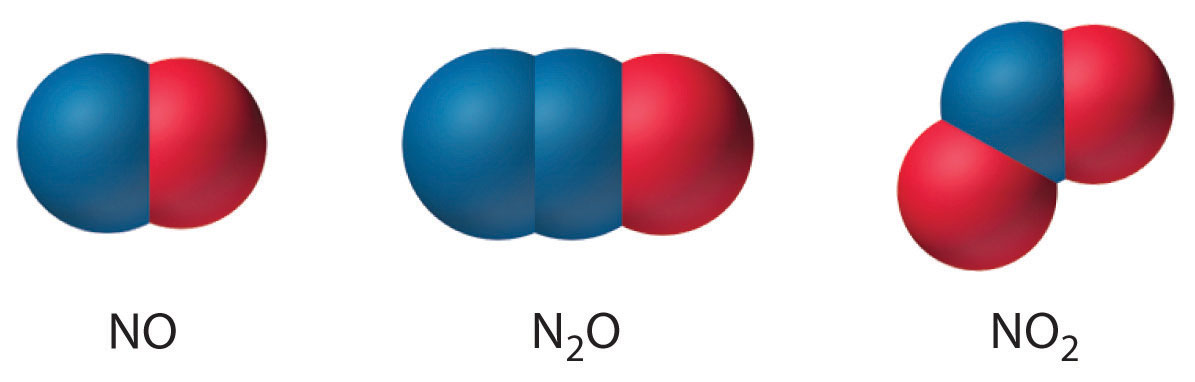
\includegraphics[width=0.6\textwidth]{../../figures/nox-molecules.jpg}
	\end{figure} 

	
	\begin{itemize}
		\pause
		\item \nox are detrimental to the environment and humans.
		
		\pause
		\item \nox  are naturally ocurring in man-made processes. E.g. Combustion.
		
		\pause
		\item Ammonia can "neutralize" \nox; producing water (\ch{H2O}) and nitrogen gas (\ch{N2}). Both harmless! - Selective catalytic reduction (SCR).
		
		\pause
		\item But ammonia is also hazardous to the environment/humans.
	\end{itemize}
	
\end{frame}

\begin{frame}
	\frametitle{Problem in a nutshell}
	\framesubtitle{Motivation}
	
	\begin{itemize}
		\pause
		\item The dosing of ammonia in the catalyst is key:
		
		\begin{itemize}
			\pause
			\item Too much ammonia: \nox  reduction will occur $\rightarrow$ Unnecessary ammonia emissions.
			\pause
			\item Too little ammonia: \nox  reduction will occur partially/will not occur $\rightarrow$ \nox  emissions.
			
		\end{itemize}
	\pause
		\item Gas sensors can be used to measure the concentrations of \nox  to aid on ammonia dosing.
		\pause
		\item However, the sensor also responds to ammonia.
		\pause
		\item Operating the sensor in a cyclic operation (e.g. temperature, gate bias) can enhance selectivity.
		
		\begin{itemize}
			\pause
			\item Different gasses react differently in different stages of the cycle.
			
		\end{itemize}
	\pause
		\item Temperature cycling.
		\pause
		\item \textbf{Frequency cycling}.
	\end{itemize}
	
\end{frame}


\begin{frame}
	\frametitle{Problem in a nutshell}
	\framesubtitle{Research questions}
	
	
\begin{enumerate}
	\pause
	\item Can frequency modulation be used to simultaneously quantify \nox and Ammonia concentrations?
	\pause
	\item Does the quality of fit vary over different prediction models?
\end{enumerate}
	
\end{frame}
%%%%%%%%%%%%%%%%%%%%%%%%%%%%%%%%%%%%%%%%%%%%%%%%%%%%%%%%%%%%%%%%%%%%%%%%%%%%%%%%%%%%%%%%%%%%%%%%%%%%%%%%%%
\section{Data}
\begin{frame}
	\frametitle{Data}
	\framesubtitle{Data description}
	
	\begin{itemize}
		\pause
		\item 3 gases:  \ch{NO}, \ch{NO2}, \ch{NH3}.
		\pause
		\item 5 possible concentrations each: 5, 10, 20, 40, 80 ppm.
		\pause
		\item 125 unique gas mixtures.
		\pause
		\item Frequency cycle: from 0.05 to 5000 Hz in 60 seconds.
		\pause
		\item Sampling rate: 4 Hz, i.e. 4 readings in one second.
		\pause
		\item Shape-defining features: \textbf{Slopes and Averages}.
		\pause
		\item Two important definitions:
		\begin{enumerate}
			\pause
			\item Mixture: an \textbf{unique} combination of gases, i.e. \textbf{no repetitions}.
			\pause
			\item Exposure: a combination of gasses \textbf{with repetition}.
		\end{enumerate}
	
\end{itemize}
\end{frame}

\begin{frame}
	\frametitle{Data}
	\framesubtitle{Data collection}
	
	\begin{figure}[!htb]
		\centering
		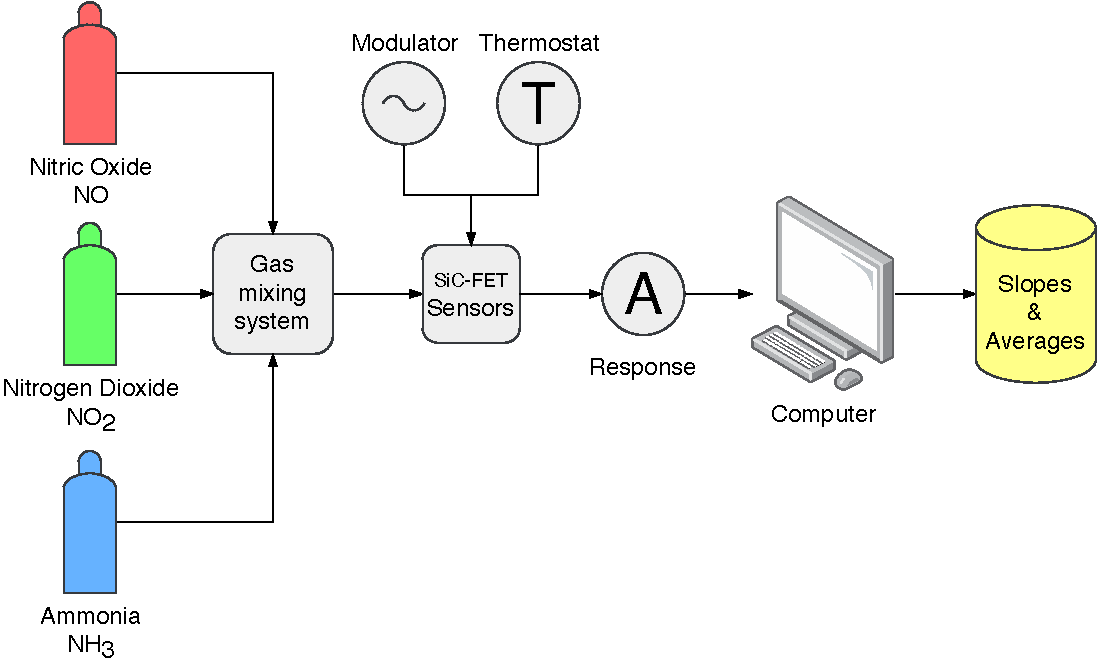
\includegraphics[width=0.8\textwidth]{../../figures/experimental-setup.pdf}
		\caption{Schema of the data acquisition process.}
	\end{figure}
\end{frame}

\begin{frame}
	\frametitle{Data}
	\framesubtitle{Data collection}
	
	\begin{figure}[!htb]
		\centering
		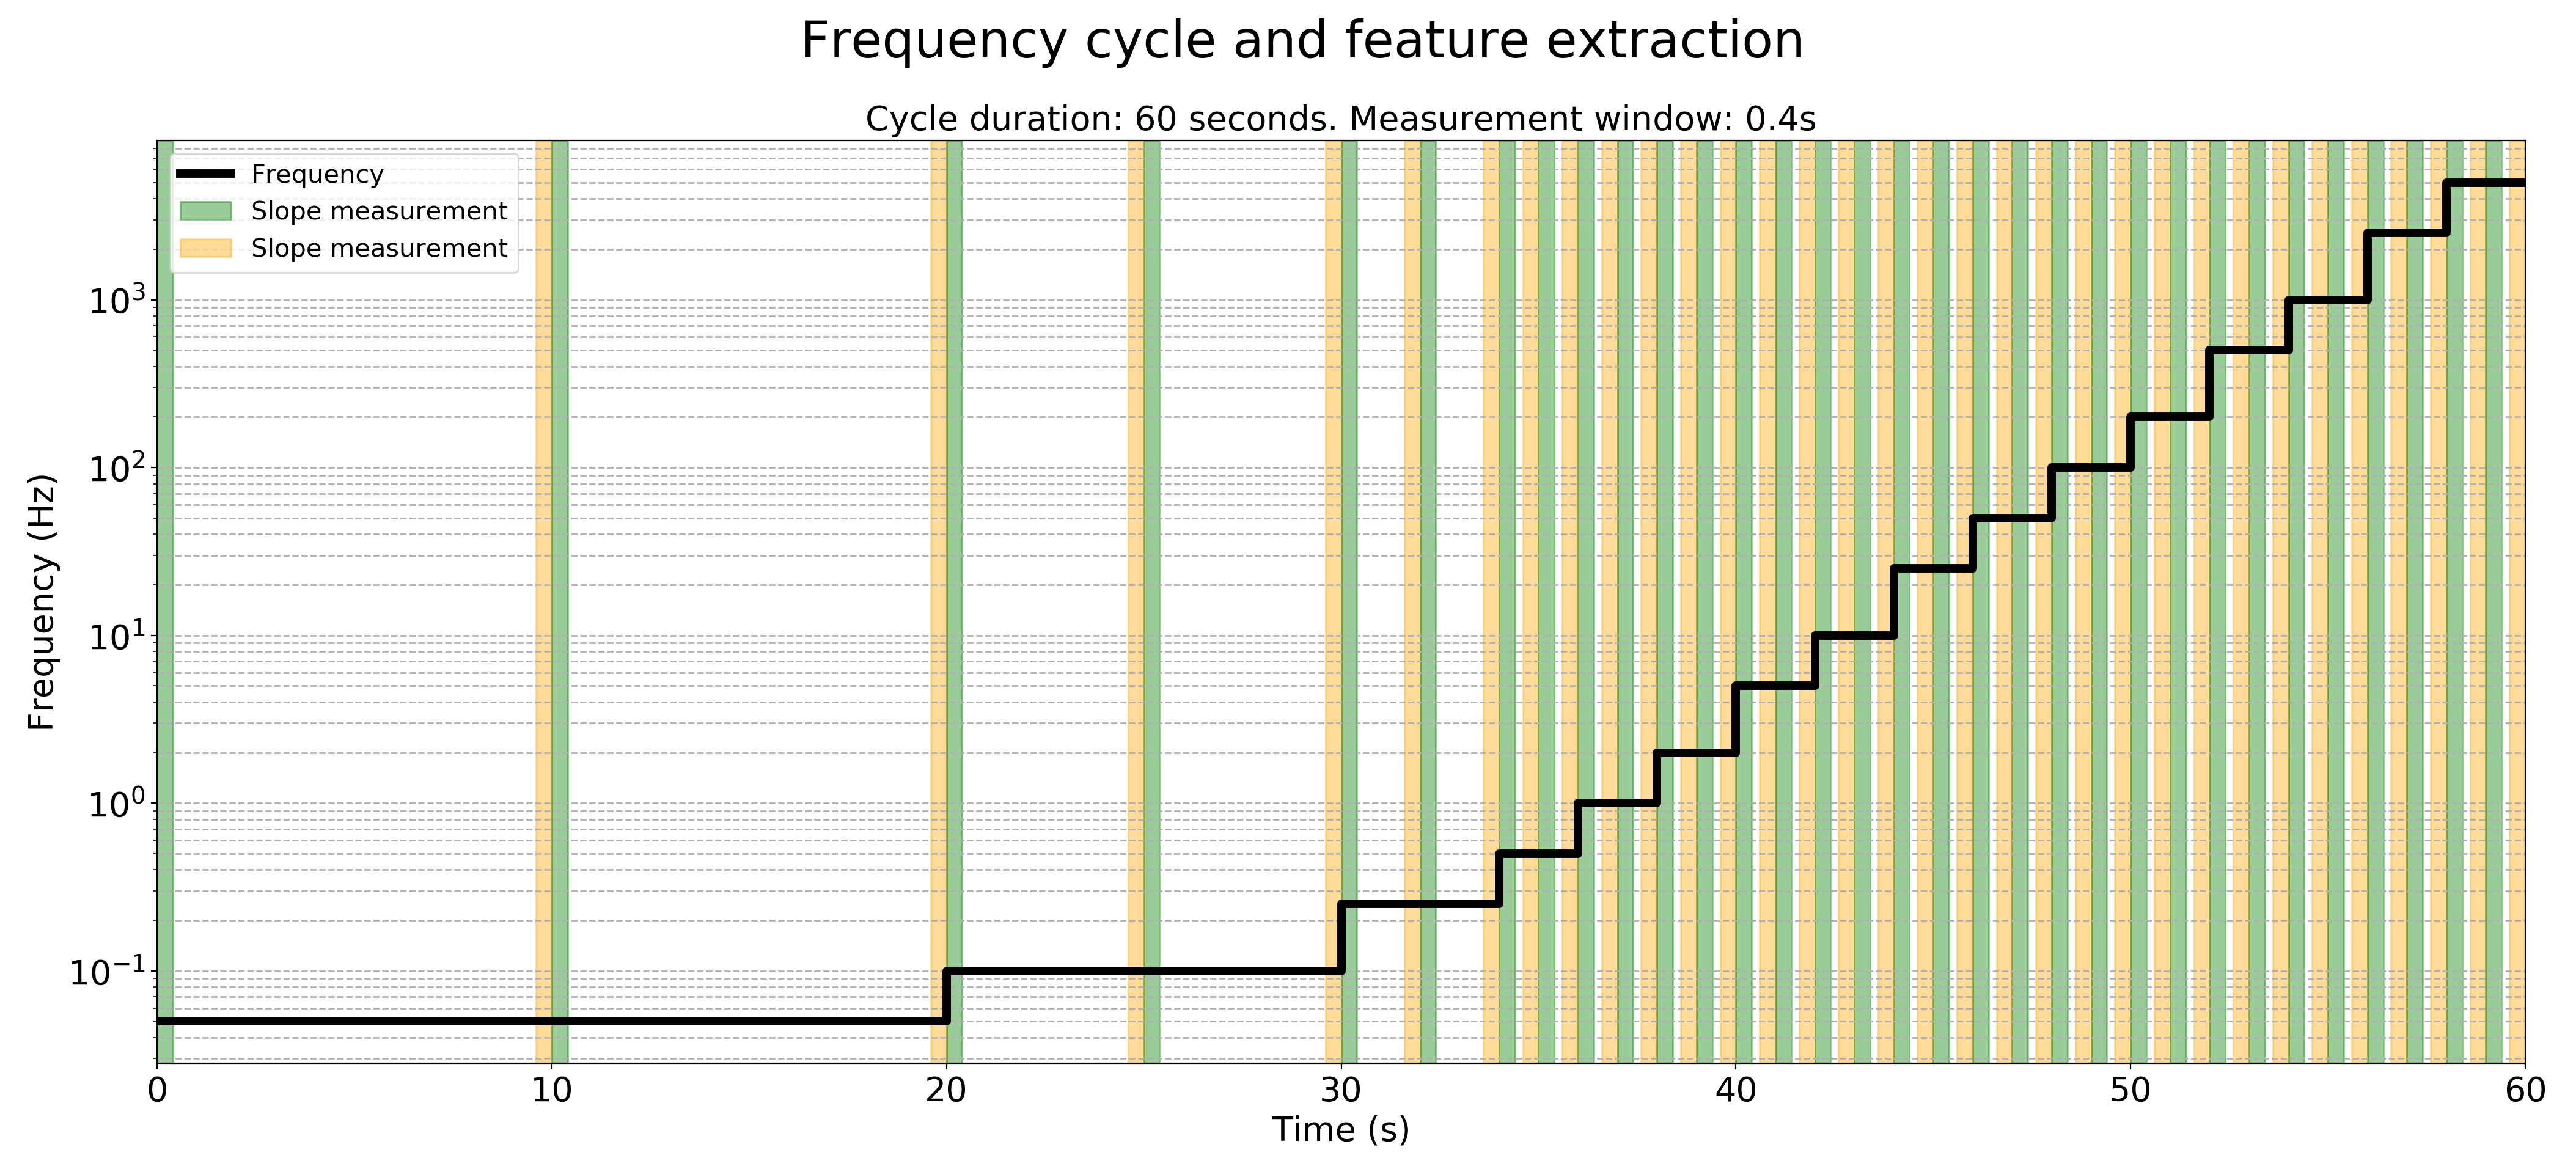
\includegraphics[width=1\textwidth]{../../figures/measurement-windows.png}
		
		\caption{Feature measurements times per cycle. The width of the red line indicates the duration of one of the feature measurement windows as an example.}
		\label{fig:feat-window}
	\end{figure} 
\end{frame}

\begin{frame}
	\frametitle{Data}
	\framesubtitle{Data collection}
	
	\begin{figure}[h]
		\centering
		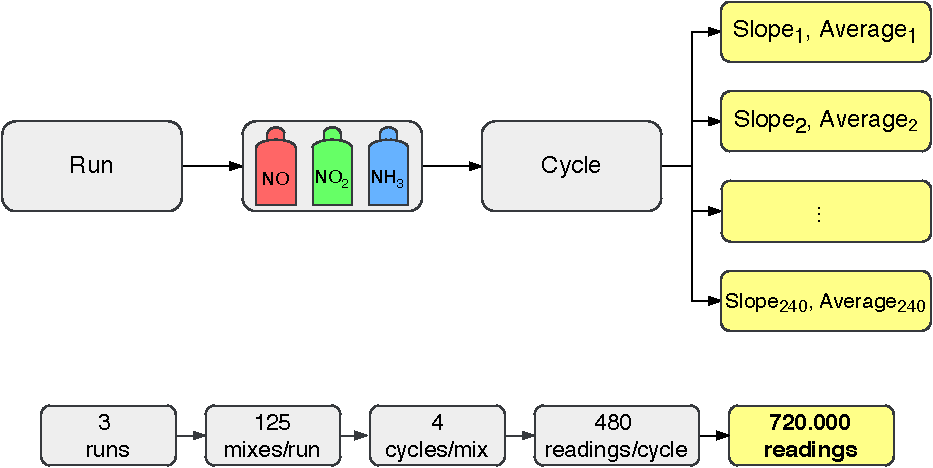
\includegraphics[width=1\textwidth]{../../figures/features.pdf}
		\caption{A visualization of the feature measurement process.}
		\label{fig:features}
	\end{figure}
\end{frame}

\begin{frame}
	\frametitle{Data}
	\framesubtitle{Raw data}
	
	Row-based
	
	\begin{table}[h]
		\centering
		\caption{Sample of raw data.}
		\label{tab:raw-sample}
		\resizebox{\textwidth}{!}{%
			\begin{tabular}{p{1.5cm}p{1.3cm}p{0.8cm}p{1.3cm}p{0.8cm}p{0.8cm}p{1.8cm}p{1.8cm}p{1.8cm}p{1.8cm}p{1.8cm}p{1.8cm}p{1.8cm}}
				\toprule[0.5mm]
				Index & Exposure\newline nr &  Cycle\newline  nr &  Sample\newline  nr &  NO\newline  [ppm] &  NO2\newline  [ppm] &  NH3\newline  [ppm] &  Freq\newline  [Hz] &  Slope\newline  sensor 1\newline [$\mu$A/s] &  Slope\newline  sensor 2\newline [$\mu$A/s] &  Average\newline  sensor 1\newline [$\mu$A] &  Average\newline  sensor 2\newline [$\mu$A] &  Sensor\newline  temperature \newline[C] \\
				\midrule[0.5mm]
				0 &            1 &         1 &          1 &        10 &          5 &         20 &       0.05 &             -18.855169 &             -22.588416 &                32.926184 &                27.961554 &              274.994683 \\
				1 &            1 &         1 &          2 &        10 &          5 &         20 &       0.05 &             -28.289268 &             -28.185027 &                25.853867 &                20.915297 &              274.980487 \\
				2 &            1 &         1 &          3 &        10 &          5 &         20 &       0.05 &              -0.390916 &              -0.482129 &                25.756138 &                20.794765 &              274.985895 \\
				3 &            1 &         1 &          4 &        10 &          5 &         20 &       0.05 &              -0.234549 &              -0.156366 &                25.697501 &                20.755673 &              275.020372 \\
				4 &            1 &         1 &          5 &        10 &          5 &         20 &       0.05 &              -0.143336 &              -0.247580 &                25.661667 &                20.693778 &              275.014964 \\
				
				\bottomrule
				&&&&&&&&&&&&\\
				&&&&&&&\sbox0{\dots}\makebox[\wd0]{\vdots}&&&&&\\
				&&&&&&&&&&&&\\
				\toprule
				
				100000 &          105 &         1 &        161 &         5 &          5 &         40 &        5.0 &             -38.366212 &             -48.495271 &                30.241896 &                24.821197 &              275.021724 \\
				100001 &          105 &         1 &        162 &         5 &          5 &         40 &        5.0 &               6.619507 &               8.521964 &                31.896773 &                26.951688 &              274.999415 \\
				100002 &          105 &         1 &        163 &         5 &          5 &         40 &        5.0 &              -1.941549 &               6.580416 &                31.411386 &                28.596792 &              275.011584 \\
				100003 &          105 &         1 &        164 &         5 &          5 &         40 &        5.0 &              27.401023 &              22.012900 &                38.261641 &                34.100017 &              275.009894 \\
				100004 &          105 &         1 &        165 &         5 &          5 &         40 &        5.0 &             -27.016623 &             -28.439121 &                31.507486 &                26.990236 &              275.014400 \\
				\bottomrule
				&&&&&&&&&&&&\\
				&&&&&&&\sbox0{\dots}\makebox[\wd0]{\vdots}&&&&&\\
				&&&&&&&&&&&&\\
				\toprule
				
				359995 &          375 &         4 &        236 &        20 &         80 &          5 &     5000.0 &              -0.136821 &              -0.158538 &                34.129879 &                30.345597 &              275.002007 \\
				359996 &          375 &         4 &        237 &        20 &         80 &          5 &     5000.0 &               0.010859 &               0.010859 &                34.132593 &                30.348312 &              274.986797 \\
				359997 &          375 &         4 &        238 &        20 &         80 &          5 &     5000.0 &              -0.043435 &               0.030405 &                34.121734 &                30.355913 &              274.979811 \\
				359998 &          375 &         4 &        239 &        20 &         80 &          5 &     5000.0 &              -0.117275 &              -0.026061 &                34.092416 &                30.349398 &              274.984543 \\
				359999 &          375 &         4 &        240 &        20 &         80 &          5 &     5000.0 &               0.073840 &               0.039092 &                34.110876 &                30.359171 &              274.998063 \\
				\bottomrule[0.5mm]
		\end{tabular}}
	\end{table}
\end{frame}


\begin{frame}
	\frametitle{Data}
	\framesubtitle{Preprocessing}
	\begin{figure}[h]
		\centering
		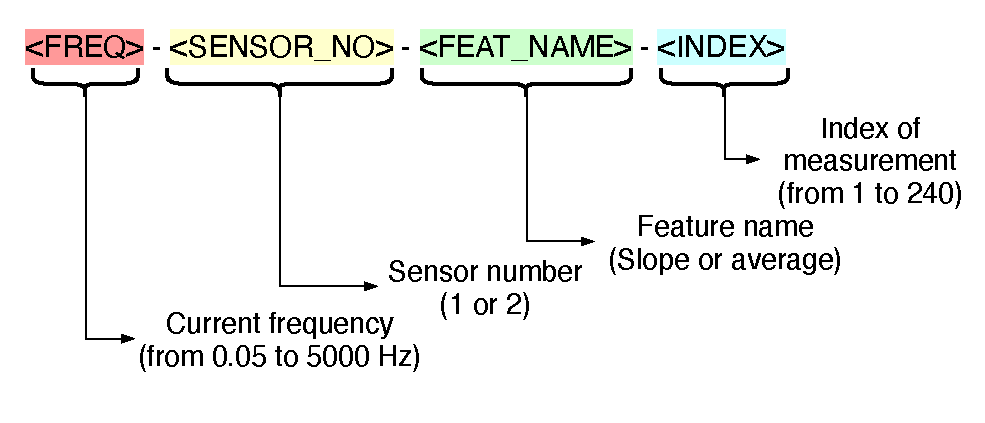
\includegraphics[width=0.6\textwidth]{../../figures/feat-naming.pdf}
		\caption{Feature naming convention.}
		\label{fig:feat-naming}
	\end{figure}

	
	\begin{figure}[h]
		\centering
		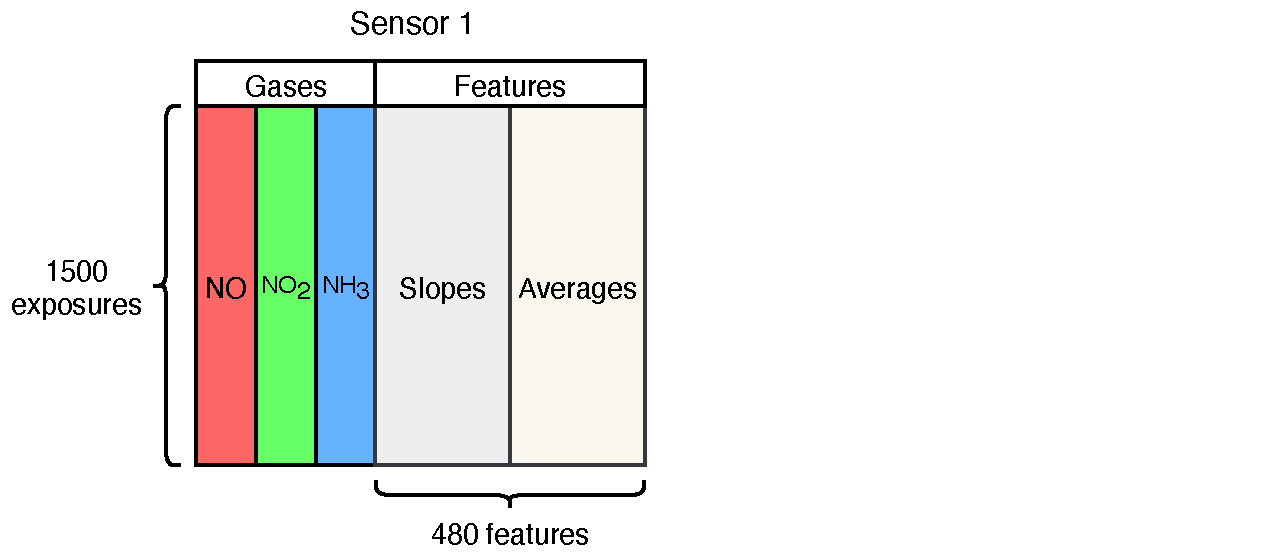
\includegraphics[width=0.35\textwidth]{../../figures/data-struct.pdf}
		\caption{Pre-processed data structure.}
		\label{fig:preprocessed-data}
	\end{figure}
\end{frame}

\begin{frame}
	\frametitle{Data}
	\framesubtitle{Preprocessed data}
	Column-based.
	
	\begin{table}
		\centering
		\caption{Sample of pre-processed data.}
		\label{tab:prepro-sample}
		\resizebox{\textwidth}{!}{%
			\begin{tabular}{ccp{0.8cm}p{0.8cm}p{0.8cm}p{1.8cm}p{1.8cm}p{0.3cm}p{1.6cm}p{1.6cm}p{1.6cm}p{1.6cm}p{0.3cm}p{1.6cm}p{1.6cm}}
				\toprule[0.5mm]
				Index &  EXPOSURE &    NO &   NO2 &   NH3 &  0.05-1-slope-0 &  0.05-1-slope-1 & $\dots$&  5000.0-1-slope-239 &  0.05-1-avg-0 &  0.05-1-avg-1 &  0.05-1-avg-2 & $\dots$&  5000.0-1-avg-238 &  5000.0-1-avg-239 \\
				\midrule[0.5mm]
				0 &       1.0 &  10.0 &   5.0 &  20.0 &      -18.855169 &      -28.289268 &$\dots$&            0.019546 &     32.926184 &     25.853867 &     25.756138 &$\dots$&         35.840135 &         35.845021 \\
				1 &       1.0 &  10.0 &   5.0 &  20.0 &      -28.979886 &       -9.251672 &$\dots$&           -0.056466 &     28.600050 &     26.287132 &     26.225237 & $\dots$&        35.884113 &         35.869996 \\
				2 &       1.0 &  10.0 &   5.0 &  20.0 &      -25.431240 &      -12.874158 &$\dots$&           -0.052122 &     29.512187 &     26.293647 &     26.238267 & $\dots$&        35.913432 &         35.900401 \\
				3 &       1.0 &  10.0 &   5.0 &  20.0 &      -30.126572 &       -8.196200 &$\dots$&           -0.156366 &     28.368758 &     26.319708 &     26.254555 &$\dots$&         35.939493 &         35.900401 \\
				4 &       2.0 &  20.0 &  40.0 &  40.0 &      -19.506695 &      -27.051368 & $\dots$&          -0.078183 &     33.180279 &     26.417437 &     26.303420 &$\dots$&         35.685397 &         35.665852 \\
				\bottomrule
				&&&&&&&&&&&&&&\\
				&&&&&&&\sbox0{\dots}\makebox[\wd0]{\vdots}&&&&&&&\\
				&&&&&&&&&&&&&&\\
				\toprule
				
				700 &     176.0 &  40.0 &  20.0 &  40.0 &      -21.011721 &      -25.822155 &$\dots$&            -0.071668 &     31.458621 &     25.003082 &     24.902639 & $\dots$&         34.554999 &         34.537082 \\
				701 &     176.0 &  40.0 &  20.0 &  40.0 &      -27.505265 &      -10.847911 &$\dots$&             0.086870 &     27.660766 &     24.948788 &     24.918927 & $\dots$&         34.504506 &         34.526224 \\
				702 &     176.0 &  40.0 &  20.0 &  40.0 &      -27.516124 &      -10.750182 &$\dots$&            -0.097729 &     27.647193 &     24.959647 &     24.928700 & $\dots$&         34.531653 &         34.507221 \\
				703 &     176.0 &  40.0 &  20.0 &  40.0 &      -27.364102 &      -10.875058 &$\dots$&             0.086870 &     27.666195 &     24.947431 &     24.935215 & $\dots$&         34.537082 &         34.558800 \\
				704 &     177.0 &  80.0 &  40.0 &  40.0 &      -20.794546 &      -26.195696 &$\dots$&             0.041263 &     31.640505 &     25.091581 &     25.088324 &$\dots$&          34.695078 &         34.705393 \\
				
				\bottomrule
				&&&&&&&&&&&&&&\\
				&&&&&&&\sbox0{\dots}\makebox[\wd0]{\vdots}&&&&&&&\\
				&&&&&&&&&&&&&&\\
				\toprule
				
				1495 &     374.0 &  80.0 &  80.0 &  40.0 &      -27.937445 &      -10.891346 &$\dots$&            -0.097729 &     27.166692 &     24.443855 &     24.392276 &$\dots$&          34.151596 &         34.127164 \\
				1496 &     375.0 &  20.0 &  80.0 &   5.0 &      -24.358394 &      -22.933723 &$\dots$&            -0.008687 &     30.315735 &     24.582305 &     24.530726 &$\dots$&          34.134765 &         34.132593 \\
				1497 &     375.0 &  20.0 &  80.0 &   5.0 &      -28.862612 &       -9.827186 &$\dots$&            -0.112931 &     26.916940 &     24.460144 &     24.410736 &$\dots$&          34.159740 &         34.131507 \\
				1498 &     375.0 &  20.0 &  80.0 &   5.0 &      -25.839531 &      -12.780772 &$\dots$&            -0.021718 &     27.671625 &     24.476432 &     24.430282 & $\dots$&         34.143452 &         34.138023 \\
				1499 &     375.0 &  20.0 &  80.0 &   5.0 &      -28.002598 &      -10.645937 &$\dots$&             0.073840 &     27.137373 &     24.475889 &     24.424853 &$\dots$&          34.092416 &         34.110876 \\
				\bottomrule[0.5mm]
		\end{tabular}}
	\end{table}
\end{frame}

\begin{frame}
	\frametitle{Data}
	\framesubtitle{Feature averaging}
	
	\begin{itemize}
		\pause
		\item 1500 exposures - hard to visualize.
		\pause
		\item Averaging all \textbf{exposures} of a particular \textbf{mixture}.
		
	\pause
	\item 125 mixtures - easier (or less hard) to visualize
	\end{itemize}

	\begin{figure}[h]
	\centering
	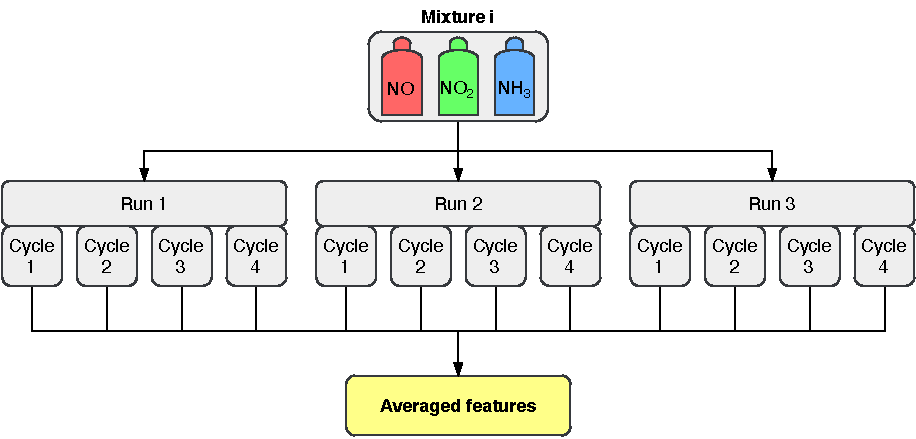
\includegraphics[width=1\textwidth]{../../figures/averaging-process.pdf}
	\caption{A visualization of the feature averaging process.}
	\label{fig:averaging-process}
\end{figure}
\end{frame}

\begin{frame}
	\frametitle{Data}
	\framesubtitle{Slopes}
		In each plot, each line represents a gas \textbf{mixture}.
		\begin{figure}[b]
			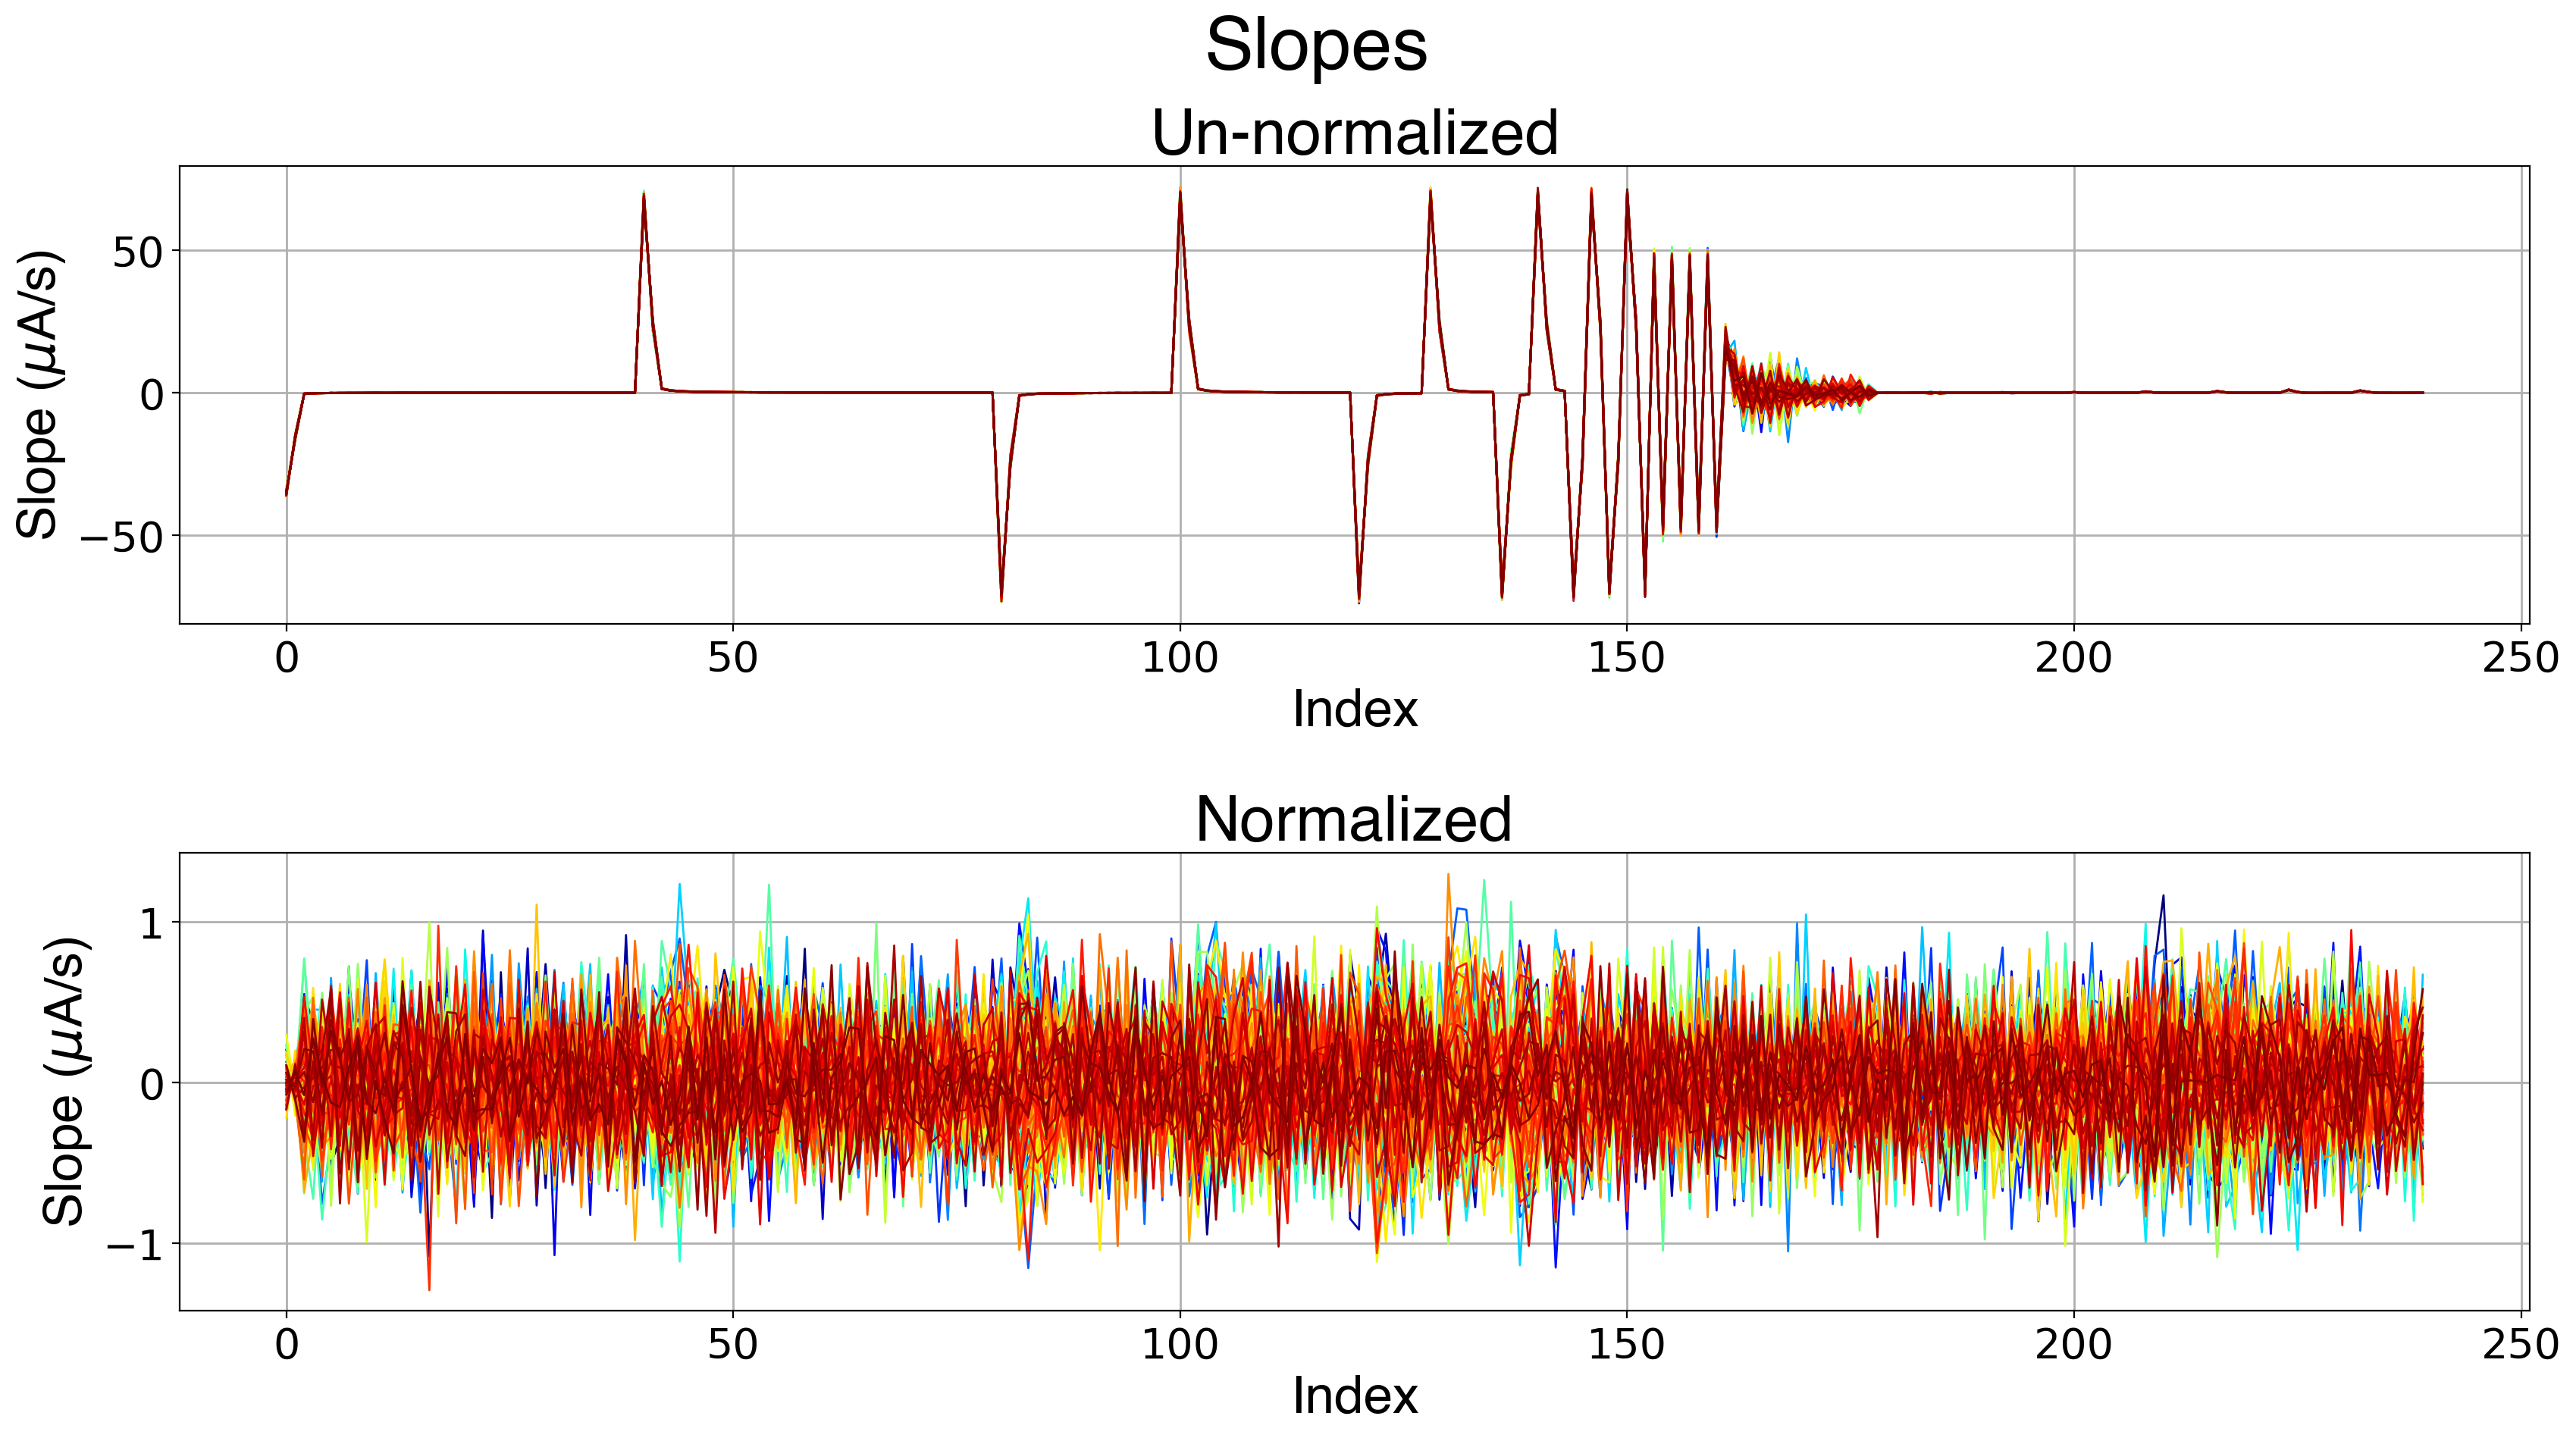
\includegraphics[width=1\linewidth]{../../figures/slopes.png}
			\caption{Slope features, un-normalized and normalized.}
			\label{fig:slopes} 
		\end{figure}
	
\end{frame}

\begin{frame}
		\frametitle{Data}
	\framesubtitle{Averages}
		In each plot, each line represents a gas \textbf{mixture}.
	\begin{figure}[b]
		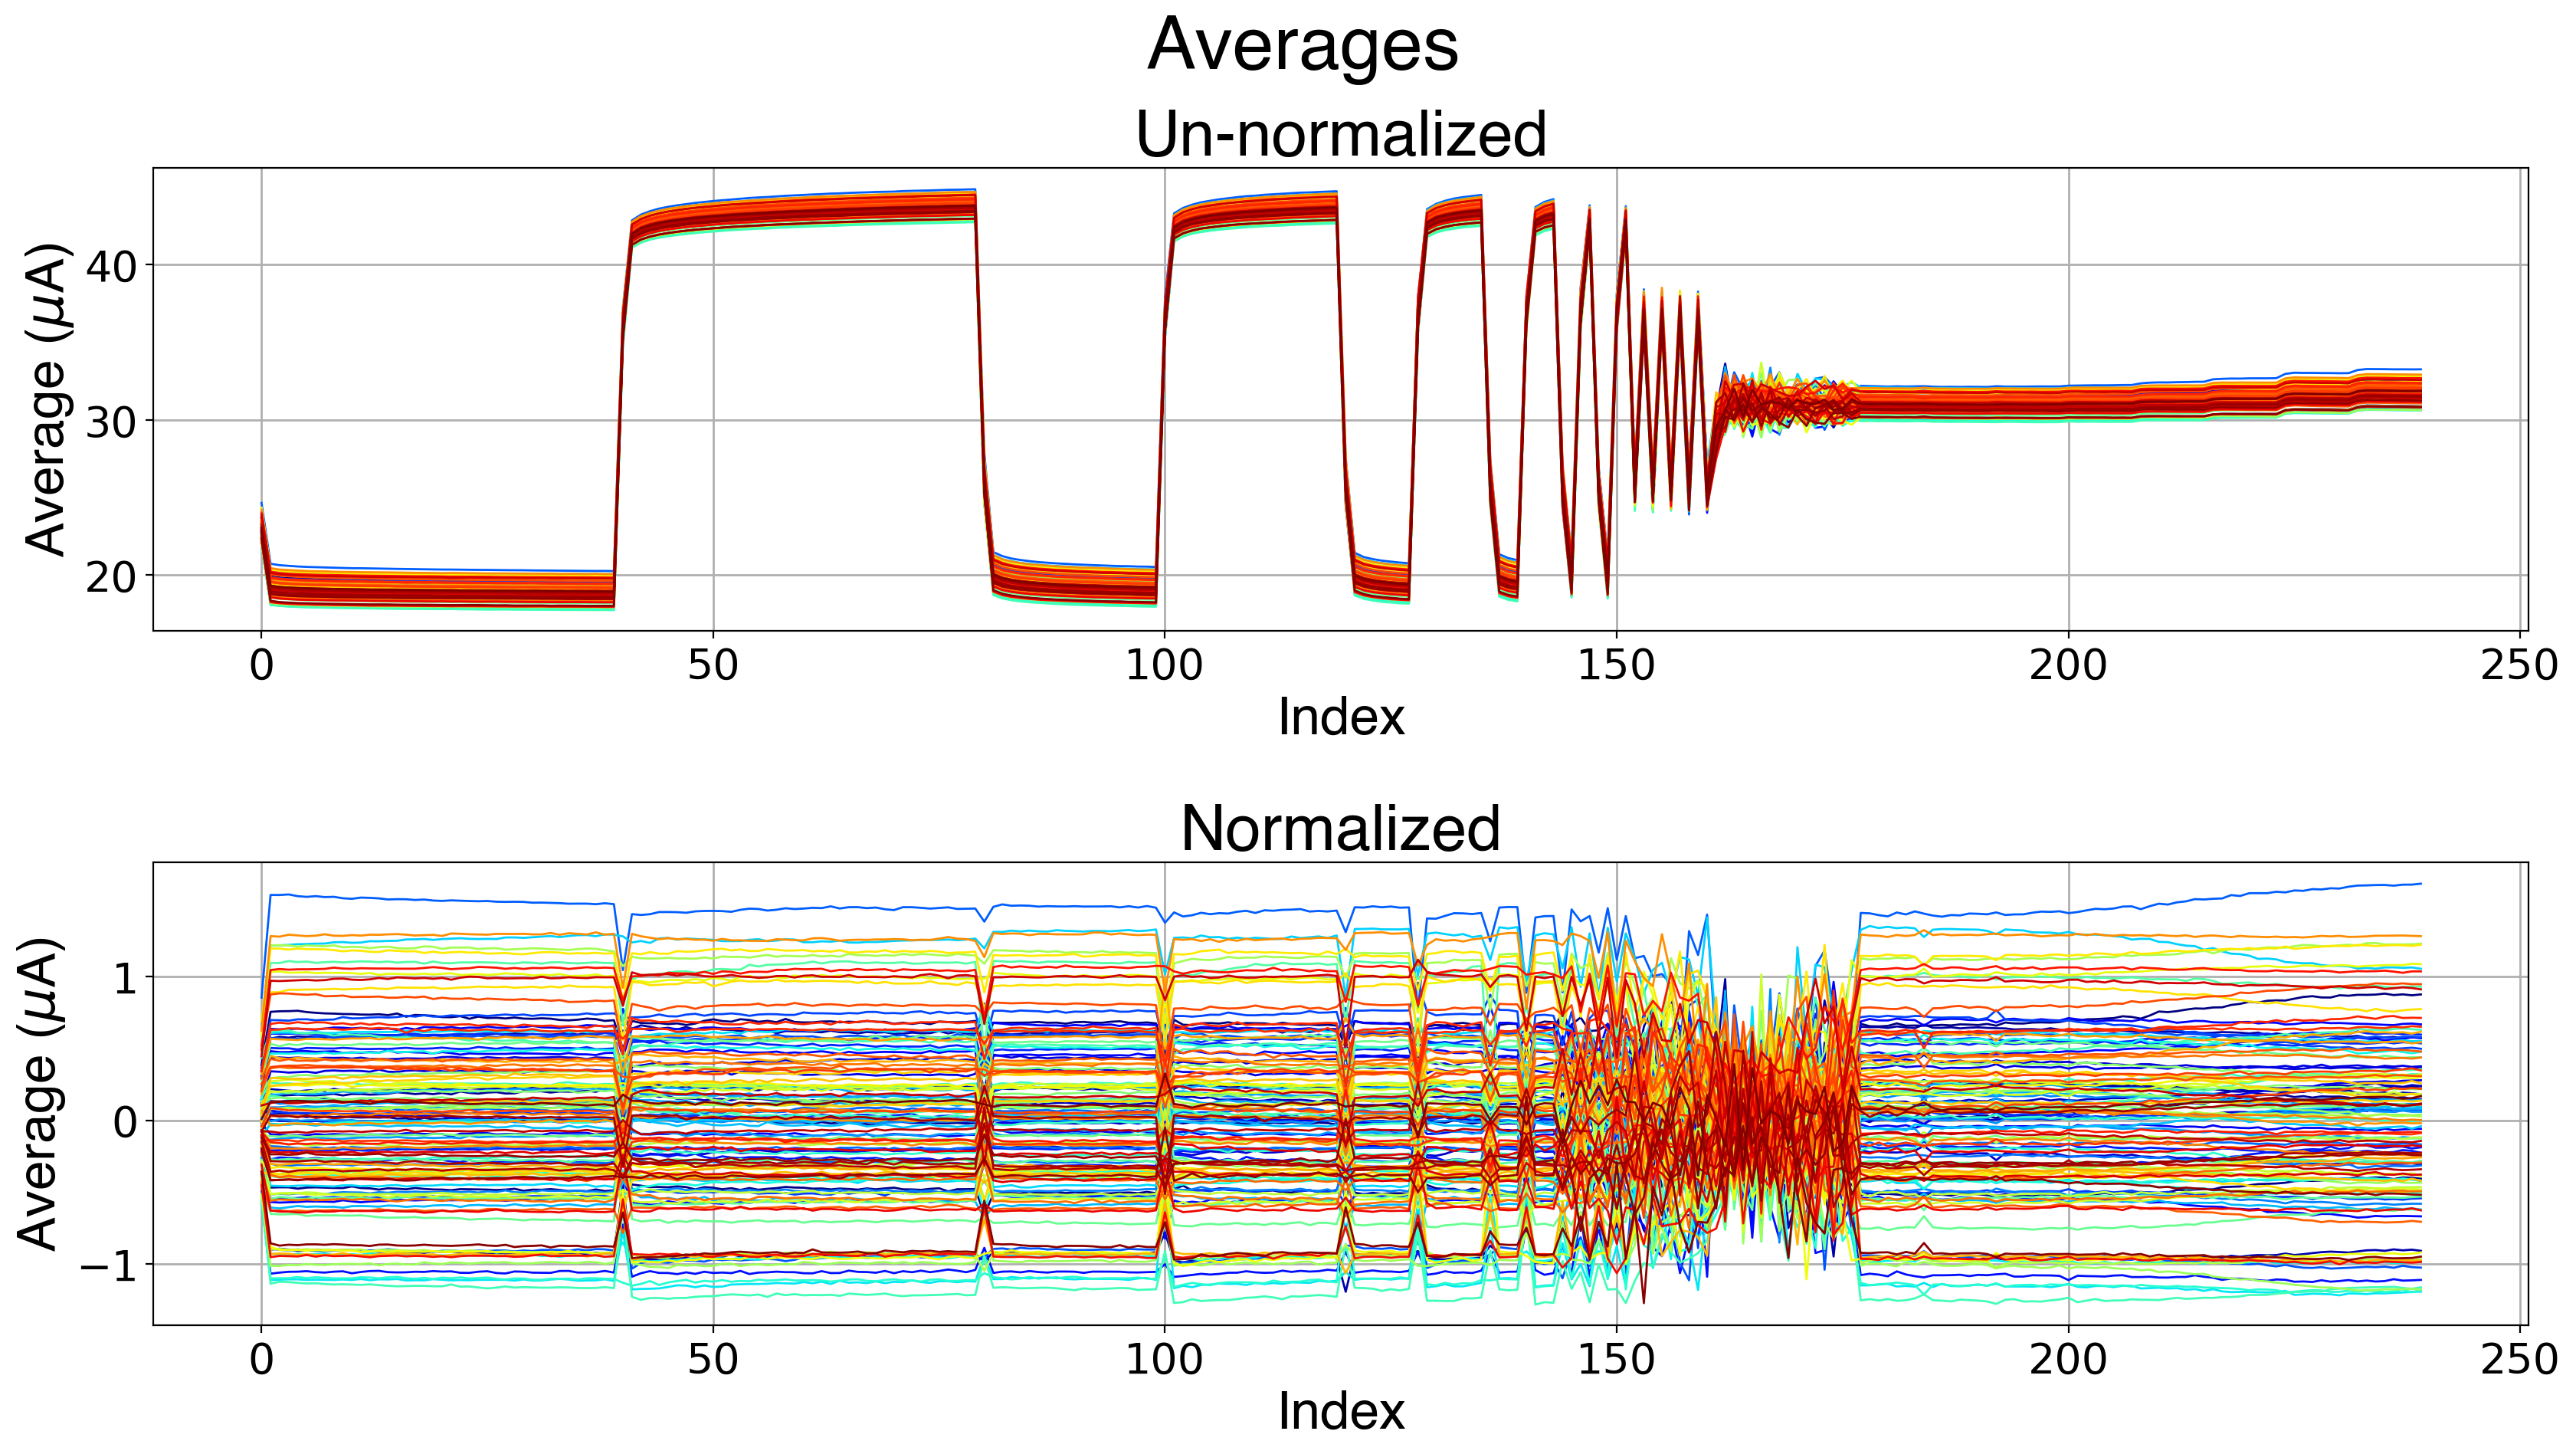
\includegraphics[width=1\linewidth]{../../figures/averages.png}
		\caption{Average features, un-normalized and normalized.}
		\label{fig:averages}
	\end{figure}
\end{frame}

\begin{frame}
	\frametitle{Data}
	\framesubtitle{Feature averaging}
	
	\begin{itemize}
		\pause
		\item Slope features don't change between mixtures (down to measuring noise).
		\pause
		\item Analysis will be \textbf{also} run on averaged averages only.
	\end{itemize}

	\begin{figure}[b]
	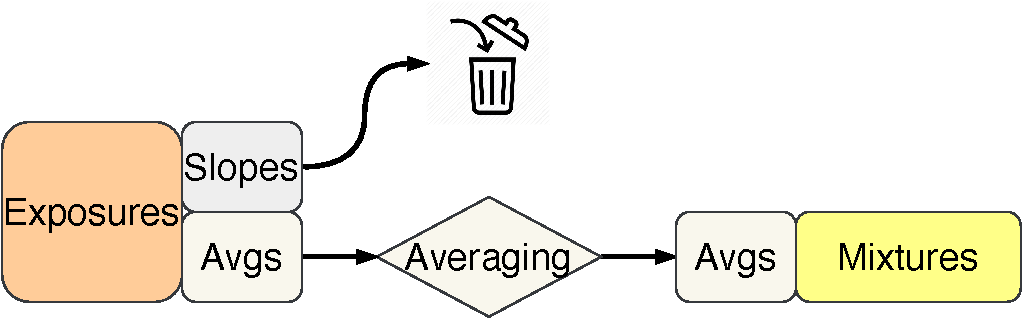
\includegraphics[width=1\linewidth]{../../figures/exp-mix.pdf}
	\end{figure}

	
\end{frame}
		



\begin{frame}
	\frametitle{Data}
	\framesubtitle{Feature averaging}
	
	\begin{table}[h]
		\centering
		\label{tab:prepro-sample-unique-mixtures}
		\resizebox{\linewidth}{!}{%
			\begin{tabular}{ccp{0.8cm}p{0.8cm}p{0.8cm}p{1.6cm}p{1.6cm}p{1.6cm}p{0.3cm}p{1.6cm}p{1.6cm}}
				\toprule[0.5mm]
				Index &  UNIQUE MIXTURE &    NO &   NO2 &   NH3 & 0.05-1-avg-0 &  0.05-1-avg-1 &  0.05-1-avg-2 & $\dots$&  5000.0-1-avg-238 &  5000.0-1-avg-239 \\
				\midrule[0.5mm]
				0 &         0 &  5.0 &  5.0 &   5.0 &  28.983749 &     25.442410 &     25.383750 &$\dots$&           35.162932 &         35.152458 \\
				1 &         1 &  5.0 &  5.0 &  10.0 & 28.538652 &     24.933269 &     24.879247 &$\dots$&           34.622460 &         34.623591 \\
				2 &         2 &  5.0 &  5.0 &  20.0 & 29.038925 &     25.245278 &     25.181935 &$\dots$&           35.025637 &         35.023103 \\
				3 &         3 &  5.0 &  5.0 &  40.0 &  28.698684 &     25.057399 &     24.980686 &$\dots$&           34.575699 &         34.576649 \\
				4 &         4 &  5.0 &  5.0 &  80.0 & 28.738748 &     25.289980 &     25.229714 & $\dots$&          34.860040 &         34.854340 \\
				\bottomrule
				&&&&&&&&&&\\
				&&&&&&&\sbox0{\dots}\makebox[\wd0]{\vdots}&&&\\
				&&&&&&&&&&\\
				\toprule
				
				70 &        70 &  20.0 &  80.0 &   5.0 &  28.142217 &     24.646824 &     24.596195 &$\dots$&         34.208650 &         34.213536 \\
				71 &        71 &  20.0 &  80.0 &  10.0 &  28.615026 &     24.952453 &     24.893228 &$\dots$&         34.511972 &         34.497900 \\
				72 &        72 &  20.0 &  80.0 &  20.0 &  28.432463 &     24.705665 &     24.649538& $\dots$&         34.317554 &         34.313437 \\
				73 &        73 &  20.0 &  80.0 &  40.0 &  28.327675 &     24.725143 &     24.685825 &$\dots$&         34.213989 &         34.197429 \\
				74 &        74 &  20.0 &  80.0 &  80.0 &  28.611836 &     25.056652 &     24.993128 &$\dots$&         34.592507 &         34.593548 \\
				
				\bottomrule
				&&&&&&&&&&\\
				&&&&&&&\sbox0{\dots}\makebox[\wd0]{\vdots}&&&\\
				&&&&&&&&&&\\
				\toprule
				
				120 &       120 &  80.0 &  80.0 &   5.0 &      28.548244 &     25.157684 &     25.103051 &$\dots$&         34.742313 &         34.749349 \\
				121 &       121 &  80.0 &  80.0 &  10.0 &    28.630183 &     25.045884 &     25.015773 & $\dots$&        34.678857 &         34.675690 \\
				122 &       122 &  80.0 &  80.0 &  20.0 &  28.420835 &     24.737087 &     24.687996 & $\dots$&        34.354338 &         34.347416 \\
				123 &       123 &  80.0 &  80.0 &  40.0 &  28.457189 &     24.743263 &     24.682929 &$\dots$&         34.327938 &         34.319839 \\
				124 &       124 &  80.0 &  80.0 &  80.0 &    28.615161 &     25.093255 &     25.046698 & $\dots$&        34.743829 &         34.734124 \\
				\bottomrule[0.5mm]
		\end{tabular}}
	\end{table}
\end{frame}




%%%%%%%%%%%%%%%%%%%%%%%%%%%%%%%%%%%%%%%%%%%%%%%%%%%%%%%%%%%%%%%%%%%%%%%%%%%%%%%%%%%%%%%%%%%%%%%%%%%%%%%%%%
\section{Methods}
\begin{frame}
	\frametitle{Methods}
	\framesubtitle{Chosen models}
	
	\begin{itemize}
		\pause
		\item Multivariate multiple regression problem
		\begin{itemize}
			\item Multiple predictors - slopes and averages.
			\item Multiple responses - gas concentrations.
		\end{itemize}
	\pause
		\item Proposed models:
		\begin{enumerate}
			\item Ordinary Least Squares Regression (OLS).
			\item Principal Components Regression (PCR).
			\item Partial Least Squares Regression (PLSR).
			\item Ridge regression.
		\end{enumerate}
	\pause
		\item Why?
			\begin{itemize}
				\pause
				\item Natural progression of model choice: simple $\rightarrow$ complex
				\pause
				\item PLSR as a starting point: shown to work well in this field/problem.
				\pause
				\item Sensor data collected in short succession: possibly high correlated features $\rightarrow$ dimensionality reduction or shrinkage to alleviate it.
			\end{itemize}
		\pause
		\item \textcolor{blue}{Pros}: backed by literature, simple to implement.
		\pause
		\item \textcolor{red}{Cons}: only linear models.
		
	\end{itemize}
	
\end{frame}

\begin{frame}
	\frametitle{Methods}
	\framesubtitle{OLS}
	
	\begin{itemize}
		\pause
	\item Relation between predictors (X) and responses (Y):

	\begin{equation}
		\label{eqn:ols}
		\mathbf{Y = XB +  E}
	\end{equation}
\pause
\item The difference between the response and the prediction is the residual. The Residual Sum of Squares is defined as:
	
	\begin{equation} 
		\label{eqn:rss}
		\text{RSS}(\mathbf{B}) = \text{Tr}[\mathbf{(Y-X\hat{B})^\intercal (Y-X\hat{B})}]
	\end{equation}
\pause
\item The estimate for coefficients $\hat{\mathbf{B}}$ is chosen to minimize the RSS:

	\begin{equation}
		\label{eqn:betahat}
		\mathbf{\hat{B}^\text{OLS}} = \underset{\mathbf{B}}{\arg\min} 	\; 	\text{RSS}(\mathbf{B})
	\end{equation}

\begin{equation}
	\label{eqn:ols_beta}
	\mathbf{\hat{B}^\text{OLS}} = \mathbf{(X^\intercal X)^{-1} X^\intercal Y}
\end{equation}
\pause
\item \small In this problem, features are sampled in quick succession (4 Hz). This will lead to highly correlated features $\rightarrow$ high variance of coefficients.
\end{itemize}
	
\end{frame}

\begin{frame}
	\frametitle{Methods}
	\framesubtitle{PCR}
	
	\begin{itemize}
	\pause
	\item The objective of PCA is to find a matrix $\mathbf{P}$ such that the linear transformation
	
		\begin{equation}
			\label{eqn:pca}
			\mathbf{T=XP^\intercal}
		\end{equation}
	
yields new variables that are uncorrelated and arranged in decreasing order of variance. The linear relation between response and PC scores is then:

	\begin{equation}
		\label{eqn:pcr}
		\mathbf{Y = T B + E}
	\end{equation}
\pause
\item And the regression coefficients are found analogously to OLS:

	\begin{equation}
		\label{eqn:beta-pcr}
		\mathbf{\hat{B}^{\text{PCR}} = (T^\intercal T)^{-1}T^\intercal Y}
	\end{equation}
\pause
\item While this method successfully best explains the variability in $\mathbf{X}$, the responses $\mathbf{Y}$ are not taken into account.
\end{itemize}
\end{frame}	

\begin{frame}
	\frametitle{Methods}
	\framesubtitle{PLSR}
	
	\begin{itemize}
	\pause
	\item Supervision of the identification of components.
	\pause
	\item Linear transformations for both $\mathbf{X}$ and $\mathbf{Y}$, analogous to PCA.
	
	\begin{equation}
	\label{eqn:x-decomp}
	\mathbf{W=XL^\intercal}
	\end{equation}

\begin{equation}
	\label{eqn:y-decomp}
	\mathbf{U = YQ^\intercal}
\end{equation}

\pause
\item The relation between responses and PLS scores is:
	\begin{equation}
	\label{eqn:plsr}
	\mathbf{Y = WB + E}
\end{equation}
\pause
\item Again, analogous to OLS, the coefficients are:

\begin{equation}
	\label{eqn:beta-plsr}
	\mathbf{\hat{B}^{\text{PLSR}} = (W^\intercal W)^{-1}W^\intercal Y}
\end{equation}
\end{itemize}
		
\end{frame}


\begin{frame}
	\frametitle{Methods}
\framesubtitle{Ridge}
\begin{itemize}


\pause
\item Shrinkage of coefficients. Coefficients tend to, but never reach, zero.
\pause
\item Addition of a regularization term.
\pause
\item $\lambda$ controls the regularization strength.
\pause
\item The RSS for multioutput ridge regression is:

\begin{equation} 
	\label{eqn:rss-ridge}
	\text{RSS}^{\text{Ridge}}(\mathbf{\hat{B}, \boldsymbol{\lambda} }) = \text{Tr} [\mathbf{(Y-X\hat{B})^\intercal (Y-X\hat{B})}] + \text{Tr}[\mathbf{\hat{B}^\intercal \hat{B}+ \boldsymbol{\lambda} I}]
\end{equation}
\pause
\item Similar to before, the estimate for $\mathbf{B}$ is found by minimizing the RSS.

\begin{equation}
	\label{eqn:ridgebetahat}
	\mathbf{\hat{B}^\text{Ridge}} = \underset{\mathbf{B}}{\arg\min} 	\; \text{RSS}^{\text{Ridge}}(\mathbf{B})
\end{equation}	
\pause
\item Solving for $\mathbf{\hat{B}}$ yields:

\begin{equation}
	\label{eqn:ridgebetahat2}
	\mathbf{\hat{B}^\text{Ridge}} = \mathbf{(X^\intercal X + \boldsymbol{\lambda}  I )^{-1} X^\intercal Y}
\end{equation}

\end{itemize}

\end{frame}

\begin{frame}
	\frametitle{Methods}
	
	\begin{figure}[h]
		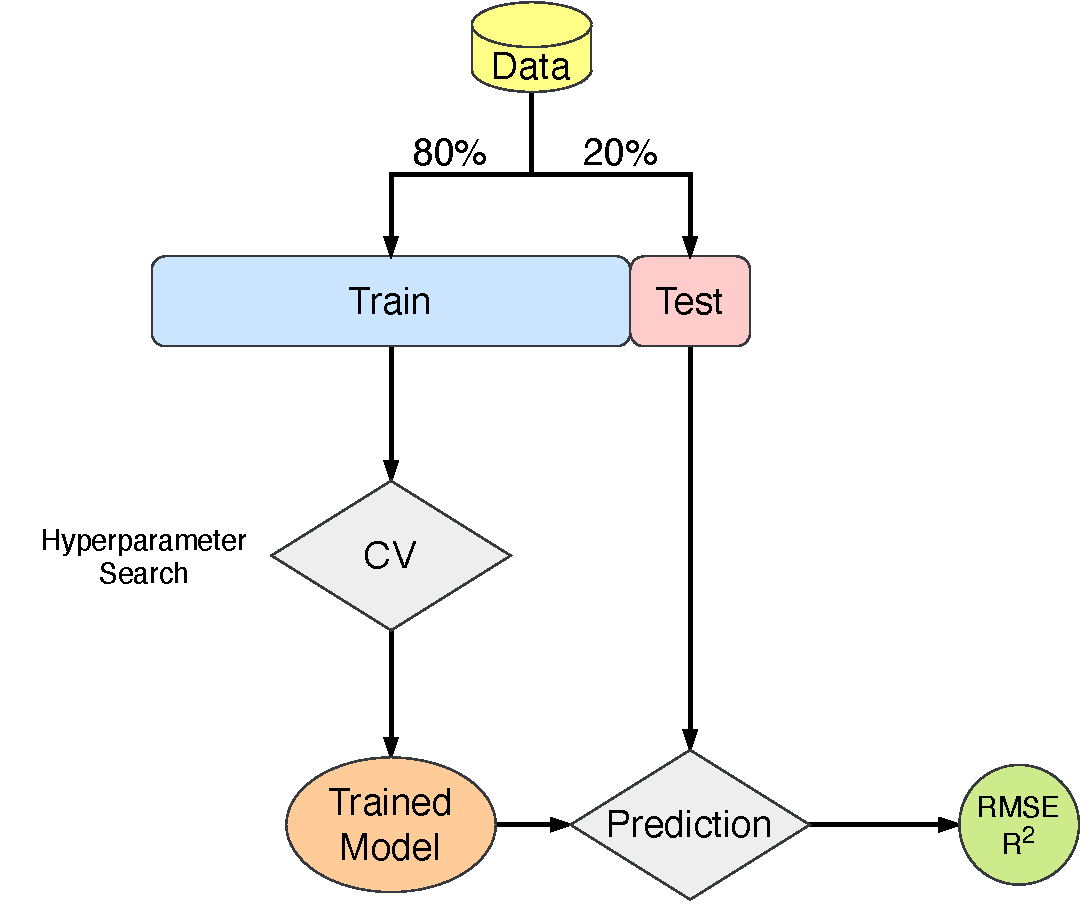
\includegraphics[width=0.7\textwidth]{../../figures/methods-schema.pdf}
	\end{figure}
	
\end{frame}
%%%%%%%%%%%%%%%%%%%%%%%%%%%%%%%%%%%%%%%%%%%%%%%%%%%%%%%%%%%%%%%%%%%%%%%%%%%%%%%%%%%%%%%%%%%%%%%%%%%%%%%%%%%5
\section{Results}
\begin{frame}
	\frametitle{Results}
	\framesubtitle{OLS}
		
		\begin{figure}[b]
			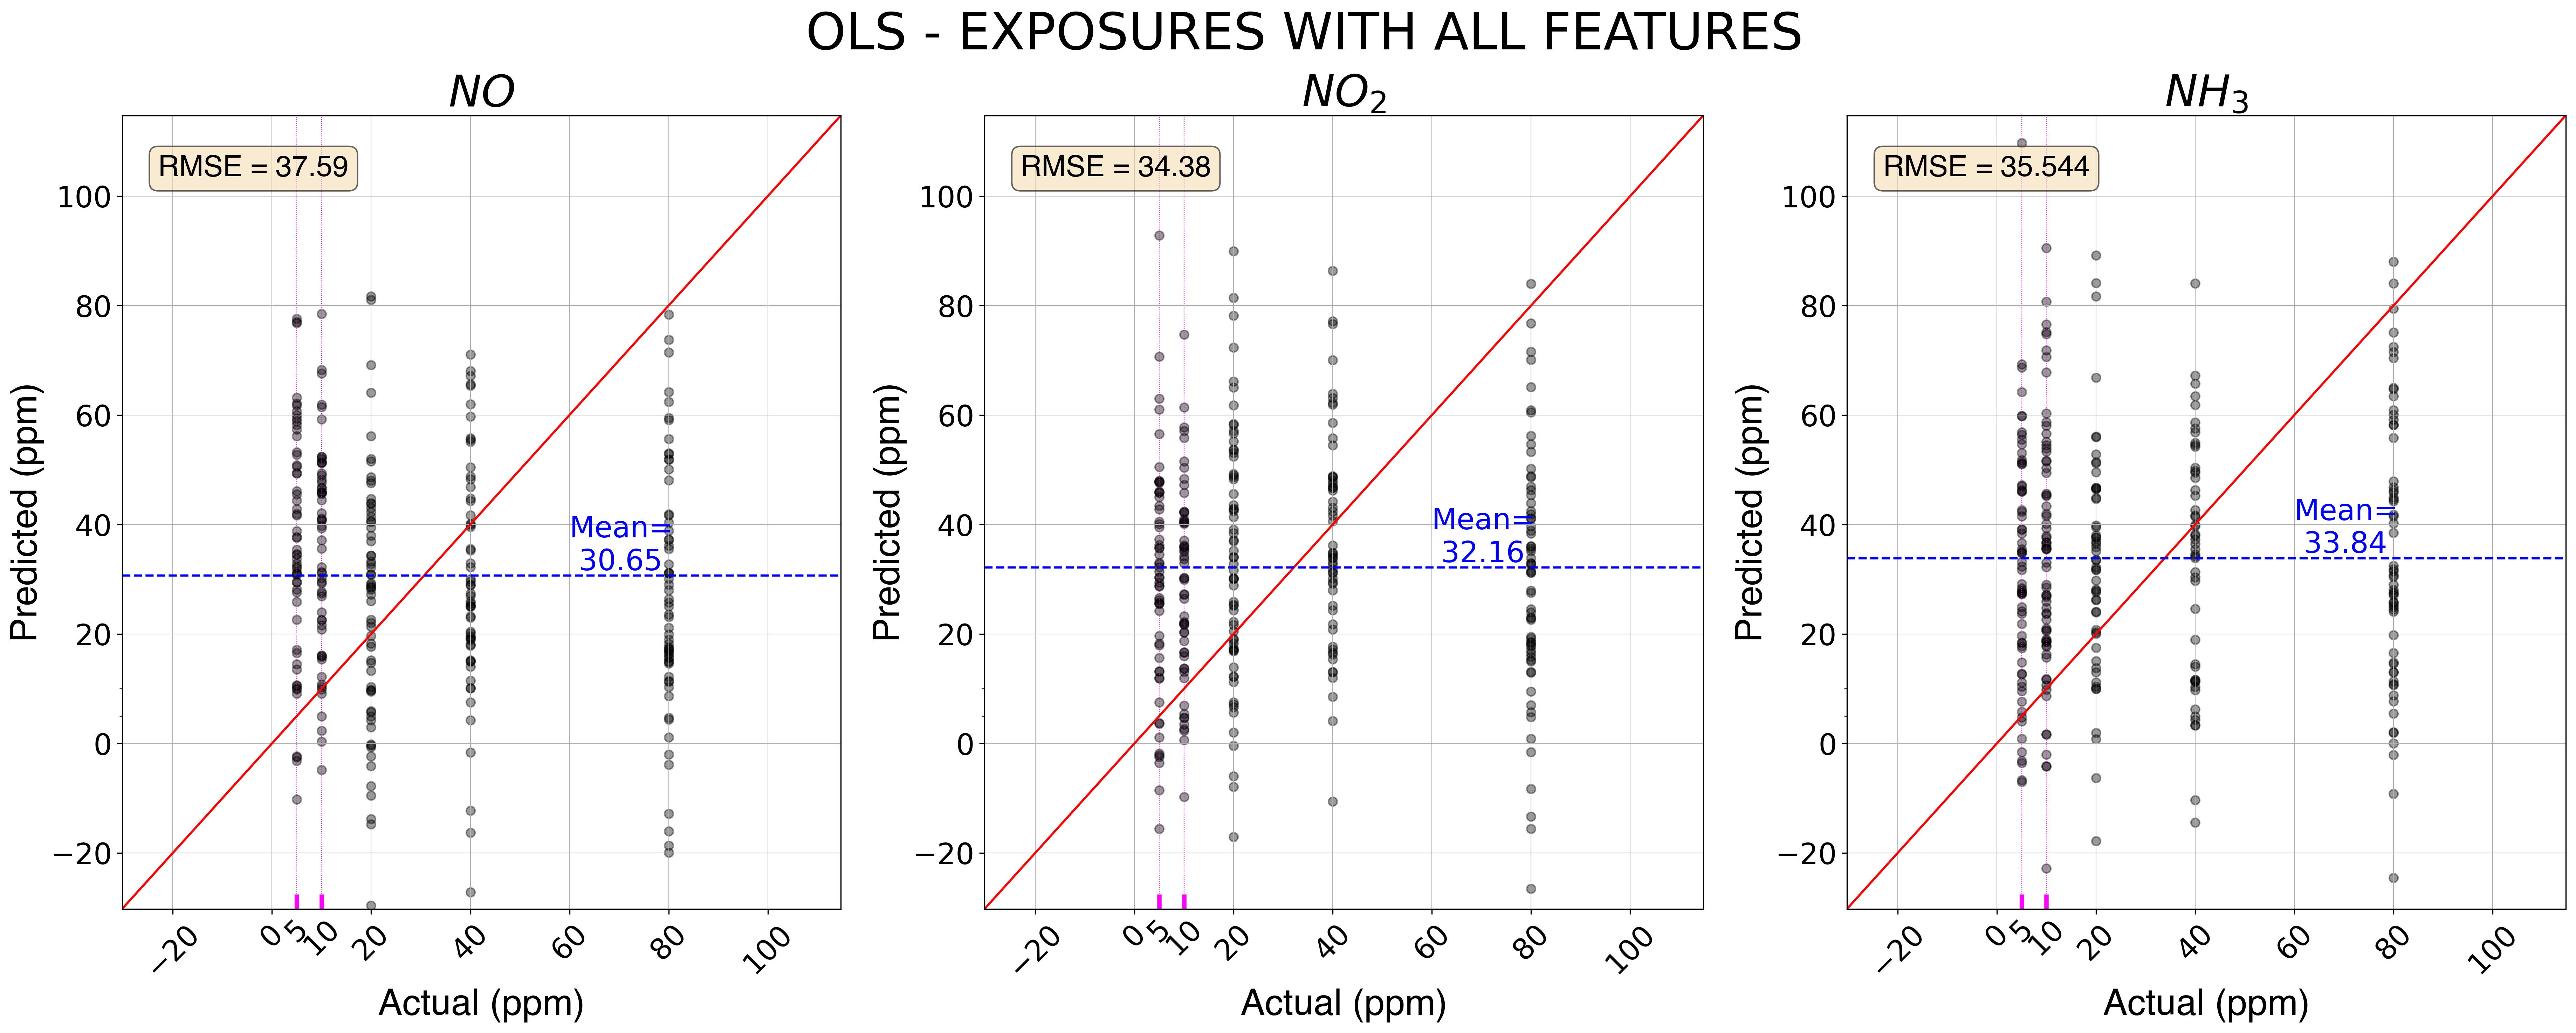
\includegraphics[width=0.8\textwidth, height = 3cm, keepaspectratio]{../../figures/ols-act-vs-pred.png}
			\caption{Actual vs. Predicted plot for \textbf{exposures}.}
			\label{fig:ols-exposures} 
		\end{figure}
		
		\begin{figure}[b]
			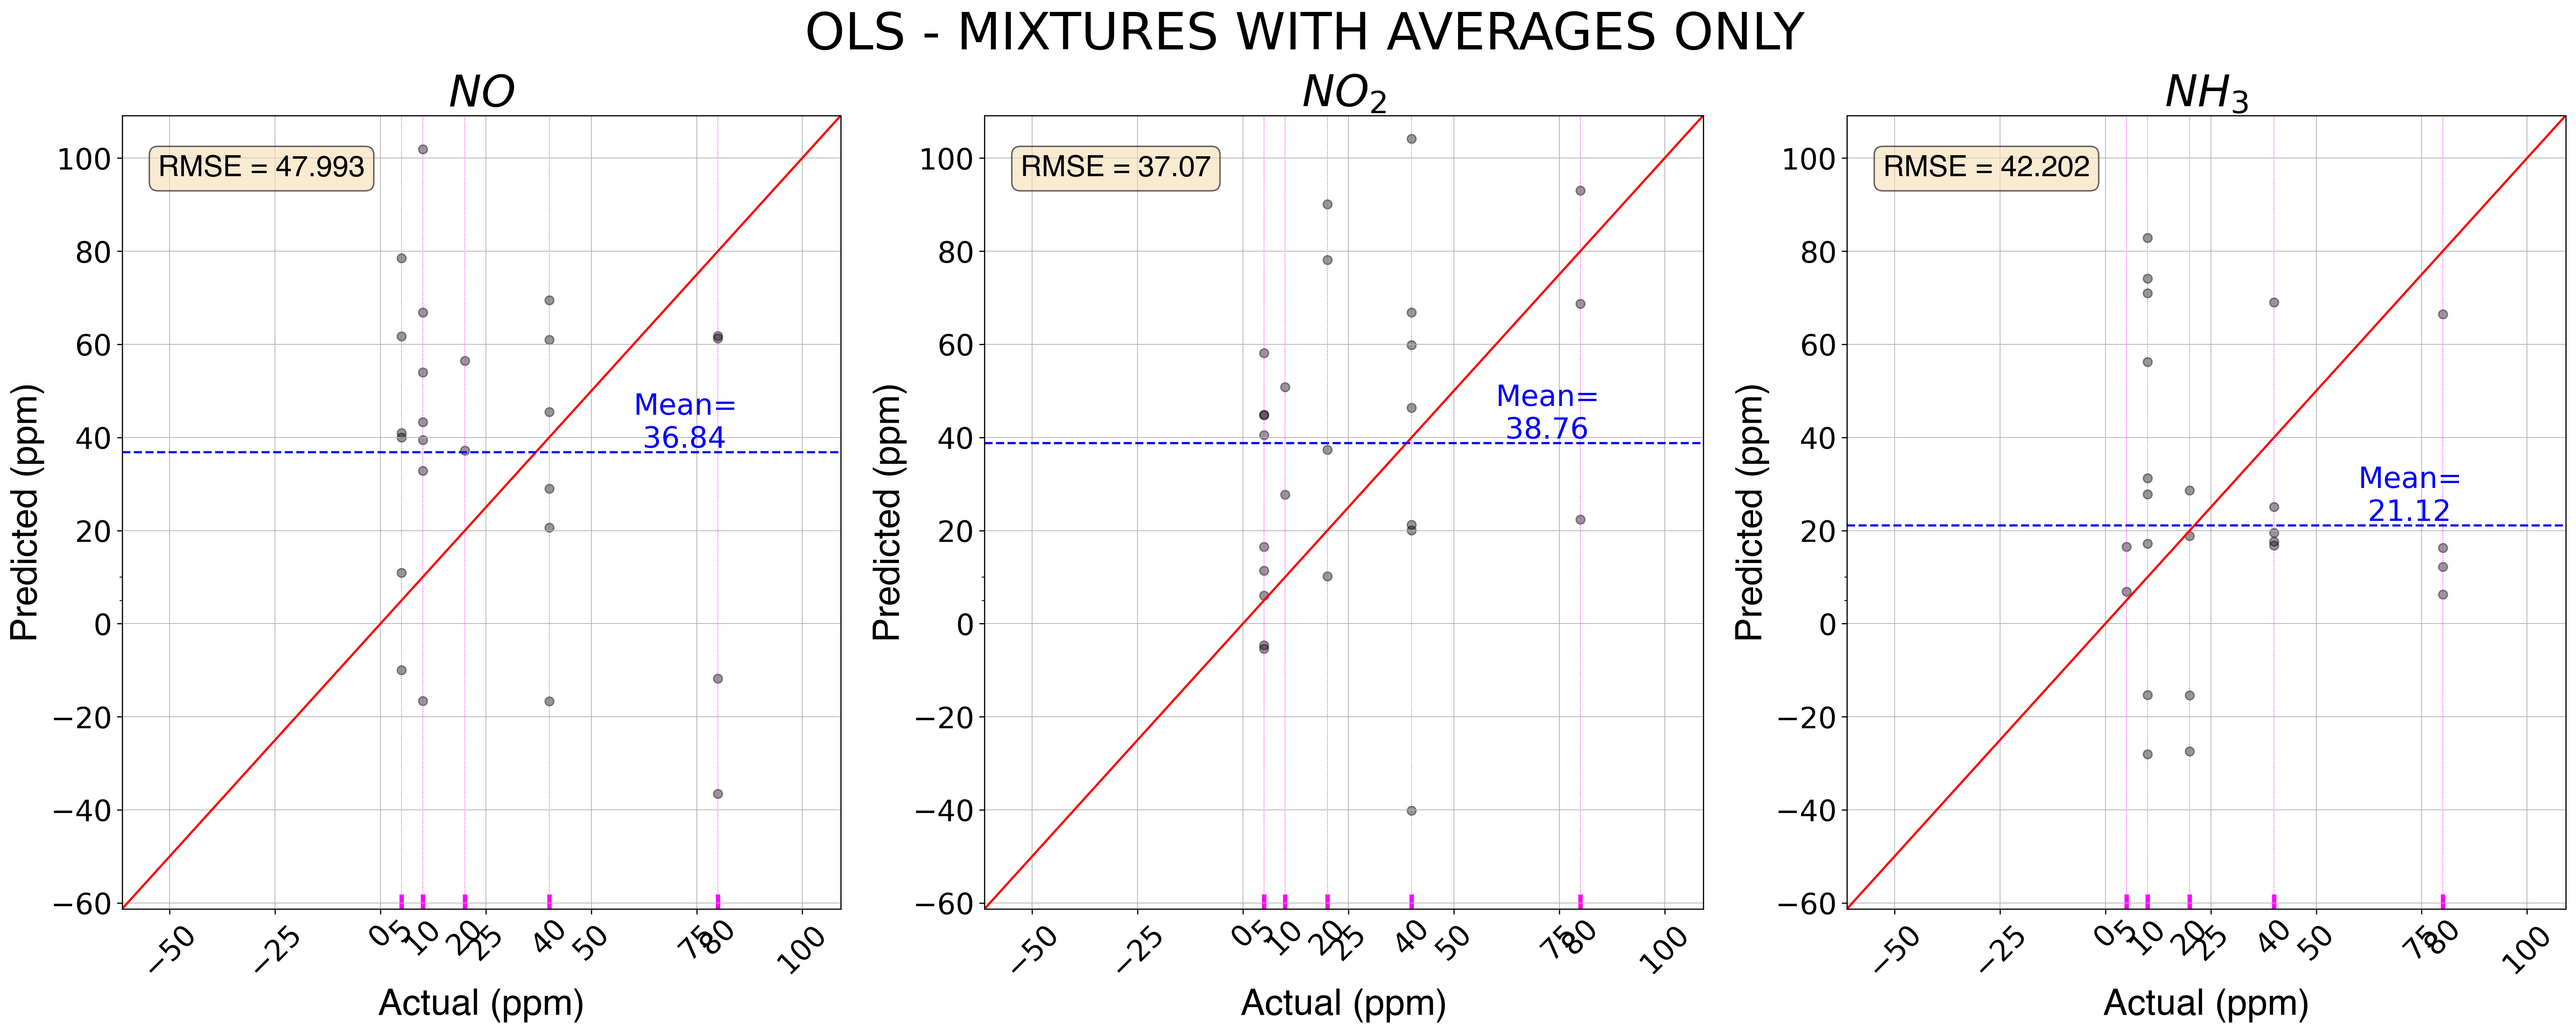
\includegraphics[width=0.8\textwidth, height = 3cm, keepaspectratio]{../../figures/ols-avg-act-vs-pred.png}
			\caption{Actual vs. Predicted plot for \textbf{mixtures} - averaged average features.}
			\label{fig:ols-averaged}
		\end{figure}
\end{frame}

\begin{frame}
	\frametitle{Results}
	\framesubtitle{PCR}
		
		\begin{figure}[h]
			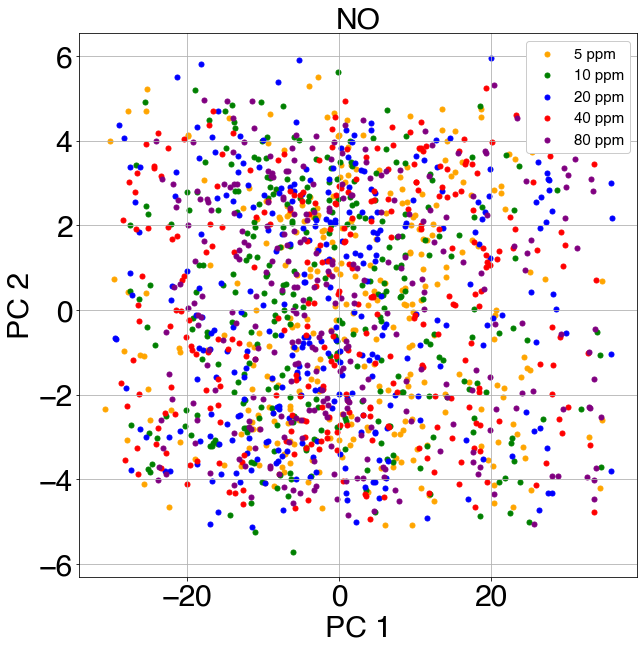
\includegraphics[width=0.30\textwidth]{../../figures/pcaNO.png}
			\hfill
			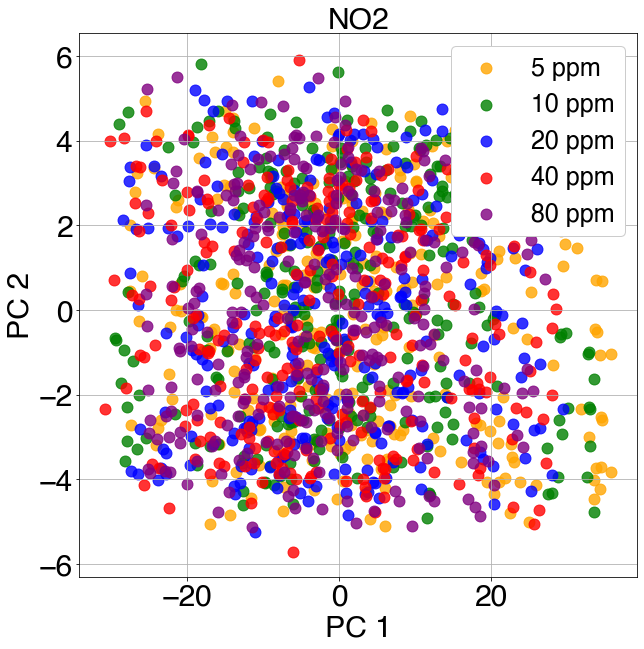
\includegraphics[width=0.30\textwidth]{../../figures/pcaNO2.png}
			\hfill
			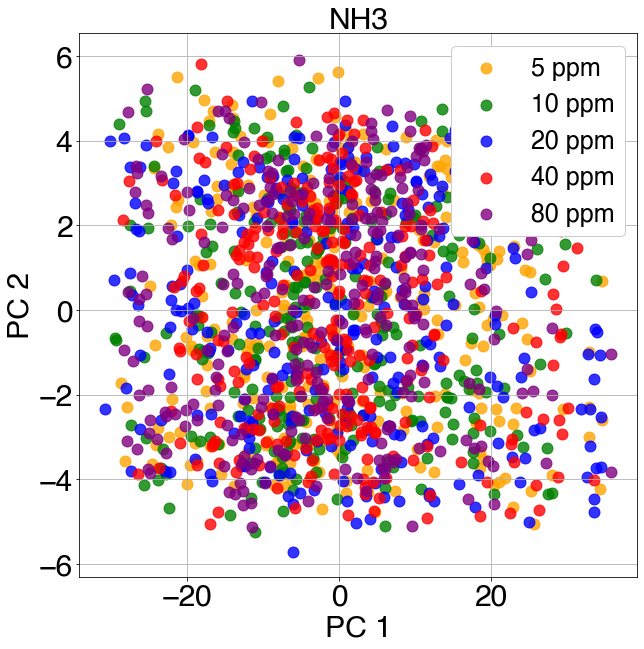
\includegraphics[width=0.30\textwidth]{../../figures/pcaNH3.png}
			\caption{PCA for slopes and averages through \textbf{exposures}}
		\end{figure}
		\begin{figure}[h]
			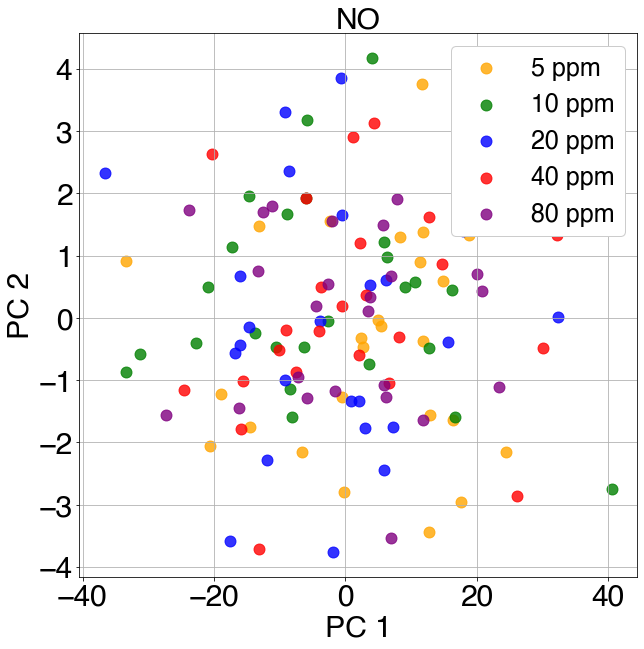
\includegraphics[width=0.30\textwidth, height = 3cm, keepaspectratio]{../../figures/pcaNO-avg-feat.png}
			\hfill
			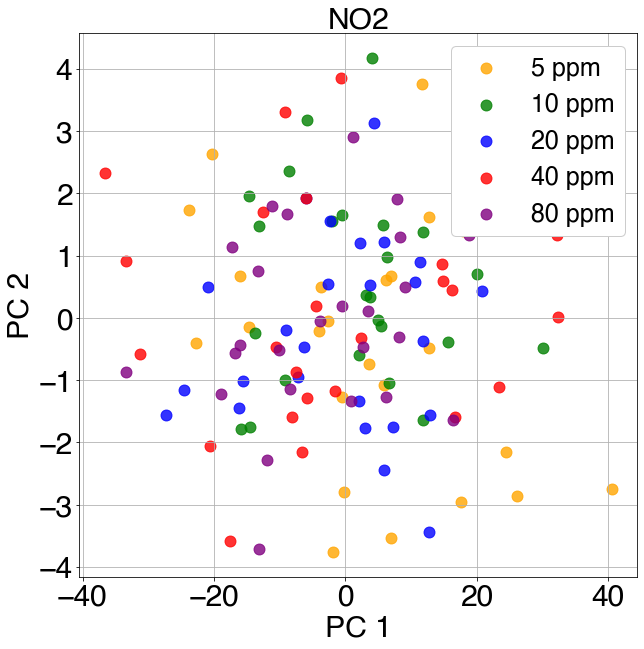
\includegraphics[width=0.30\textwidth, height = 3cm, keepaspectratio]{../../figures/pcaNO2-avg-feat.png}
			\hfill
			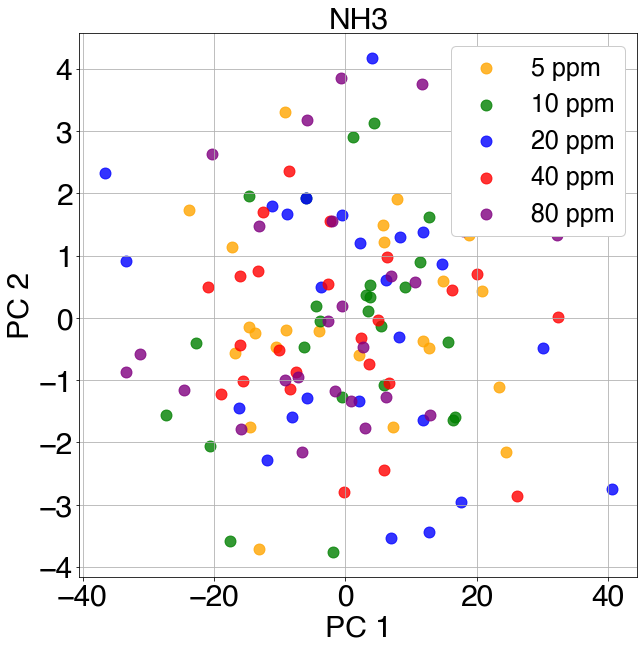
\includegraphics[width=0.30\textwidth, height = 3cm, keepaspectratio]{../../figures/pcaNH3-avg-feat.png}
			\caption{PCA for averaged average features through \textbf{mixtures}}
		\end{figure}
		
\end{frame}


\begin{frame}
	\frametitle{Results}
	\framesubtitle{PCR}
		
		\begin{figure}[t]
			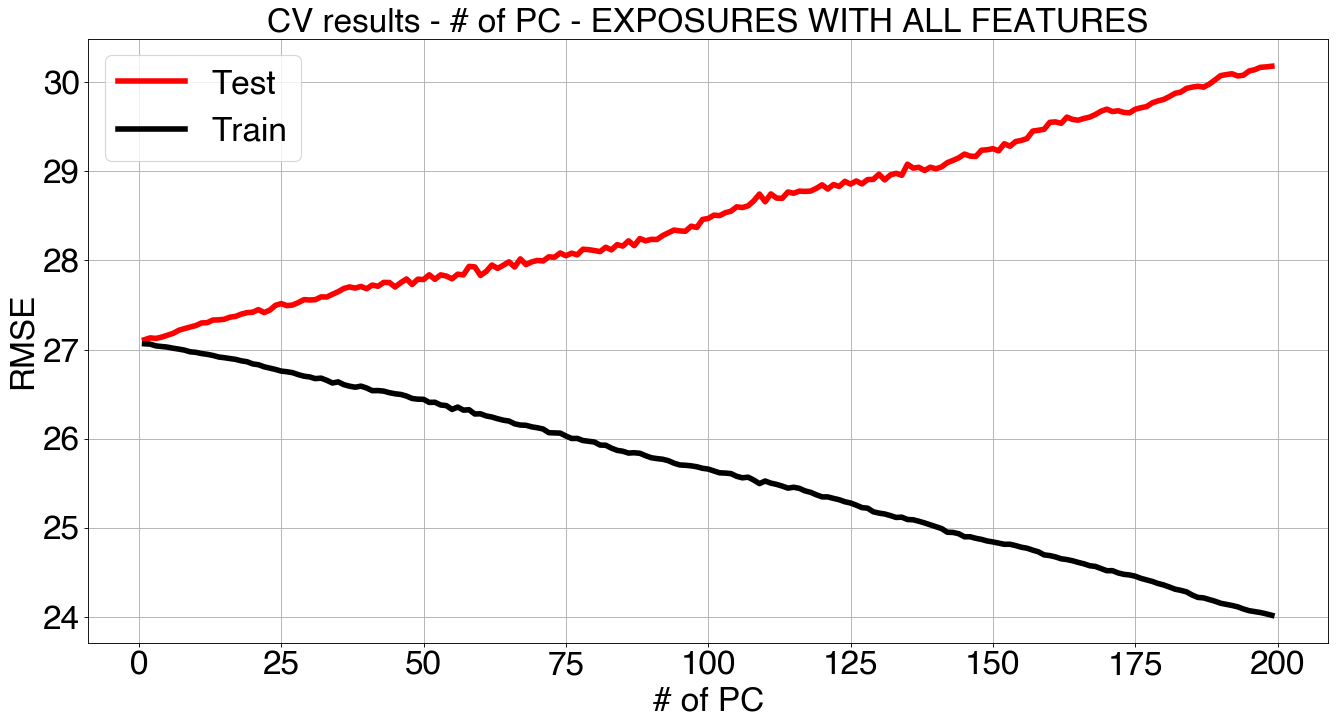
\includegraphics[width=0.5\linewidth]{../../figures/pcr-cv.png}
			\caption{CV results for \textbf{exposures}.}
			\label{fig:pcr-cv} 
		\end{figure}
		
		\begin{figure}[t]
			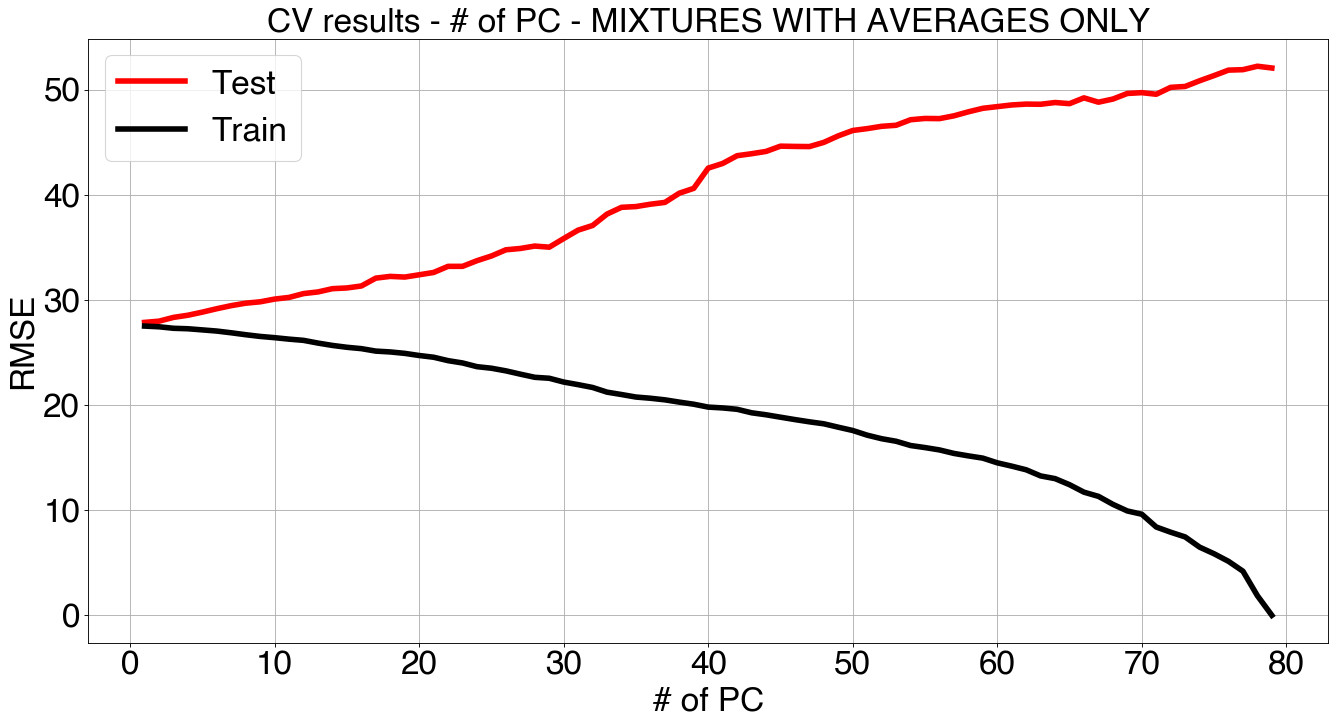
\includegraphics[width=0.5\linewidth]{../../figures/pcr-cv-avg-feat.png}
			\caption{CV results for \textbf{mixtures}.}
			\label{fig:pcr-cv-averaged}
		\end{figure}
	
\end{frame}



\begin{frame}
	\frametitle{Results}
	\framesubtitle{PCR}

		
		\begin{figure}
			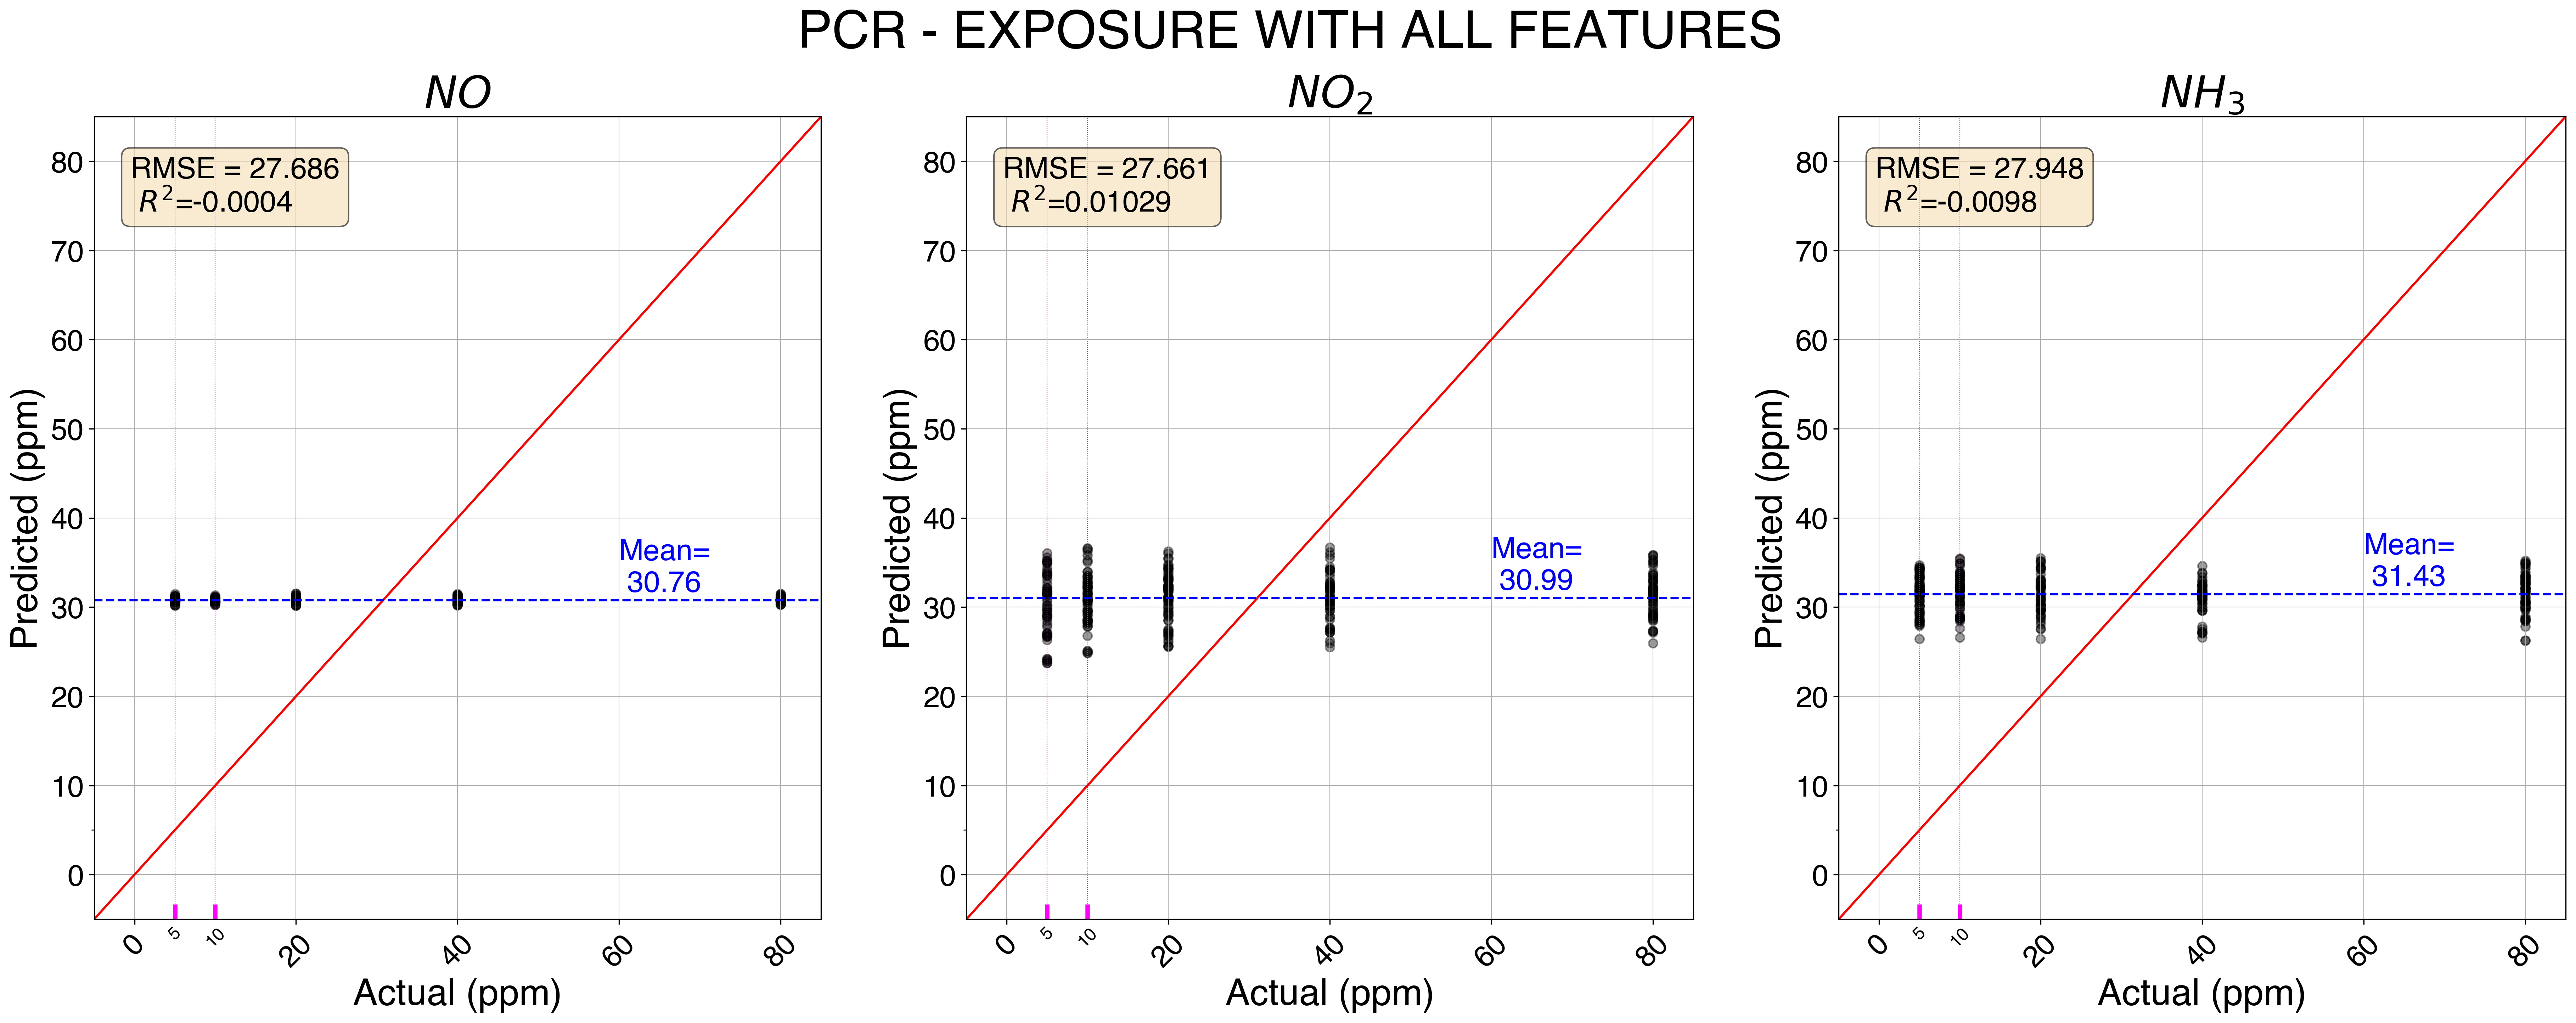
\includegraphics[width=0.8\textwidth, height = 3cm, keepaspectratio]{../../figures/pcr-act-vs-pred.png}
			\caption{Actual vs. pred for \textbf{exposures}.}
			\label{fig:pcr-act-vs-pred} 
		\end{figure}
		
		\begin{figure}
			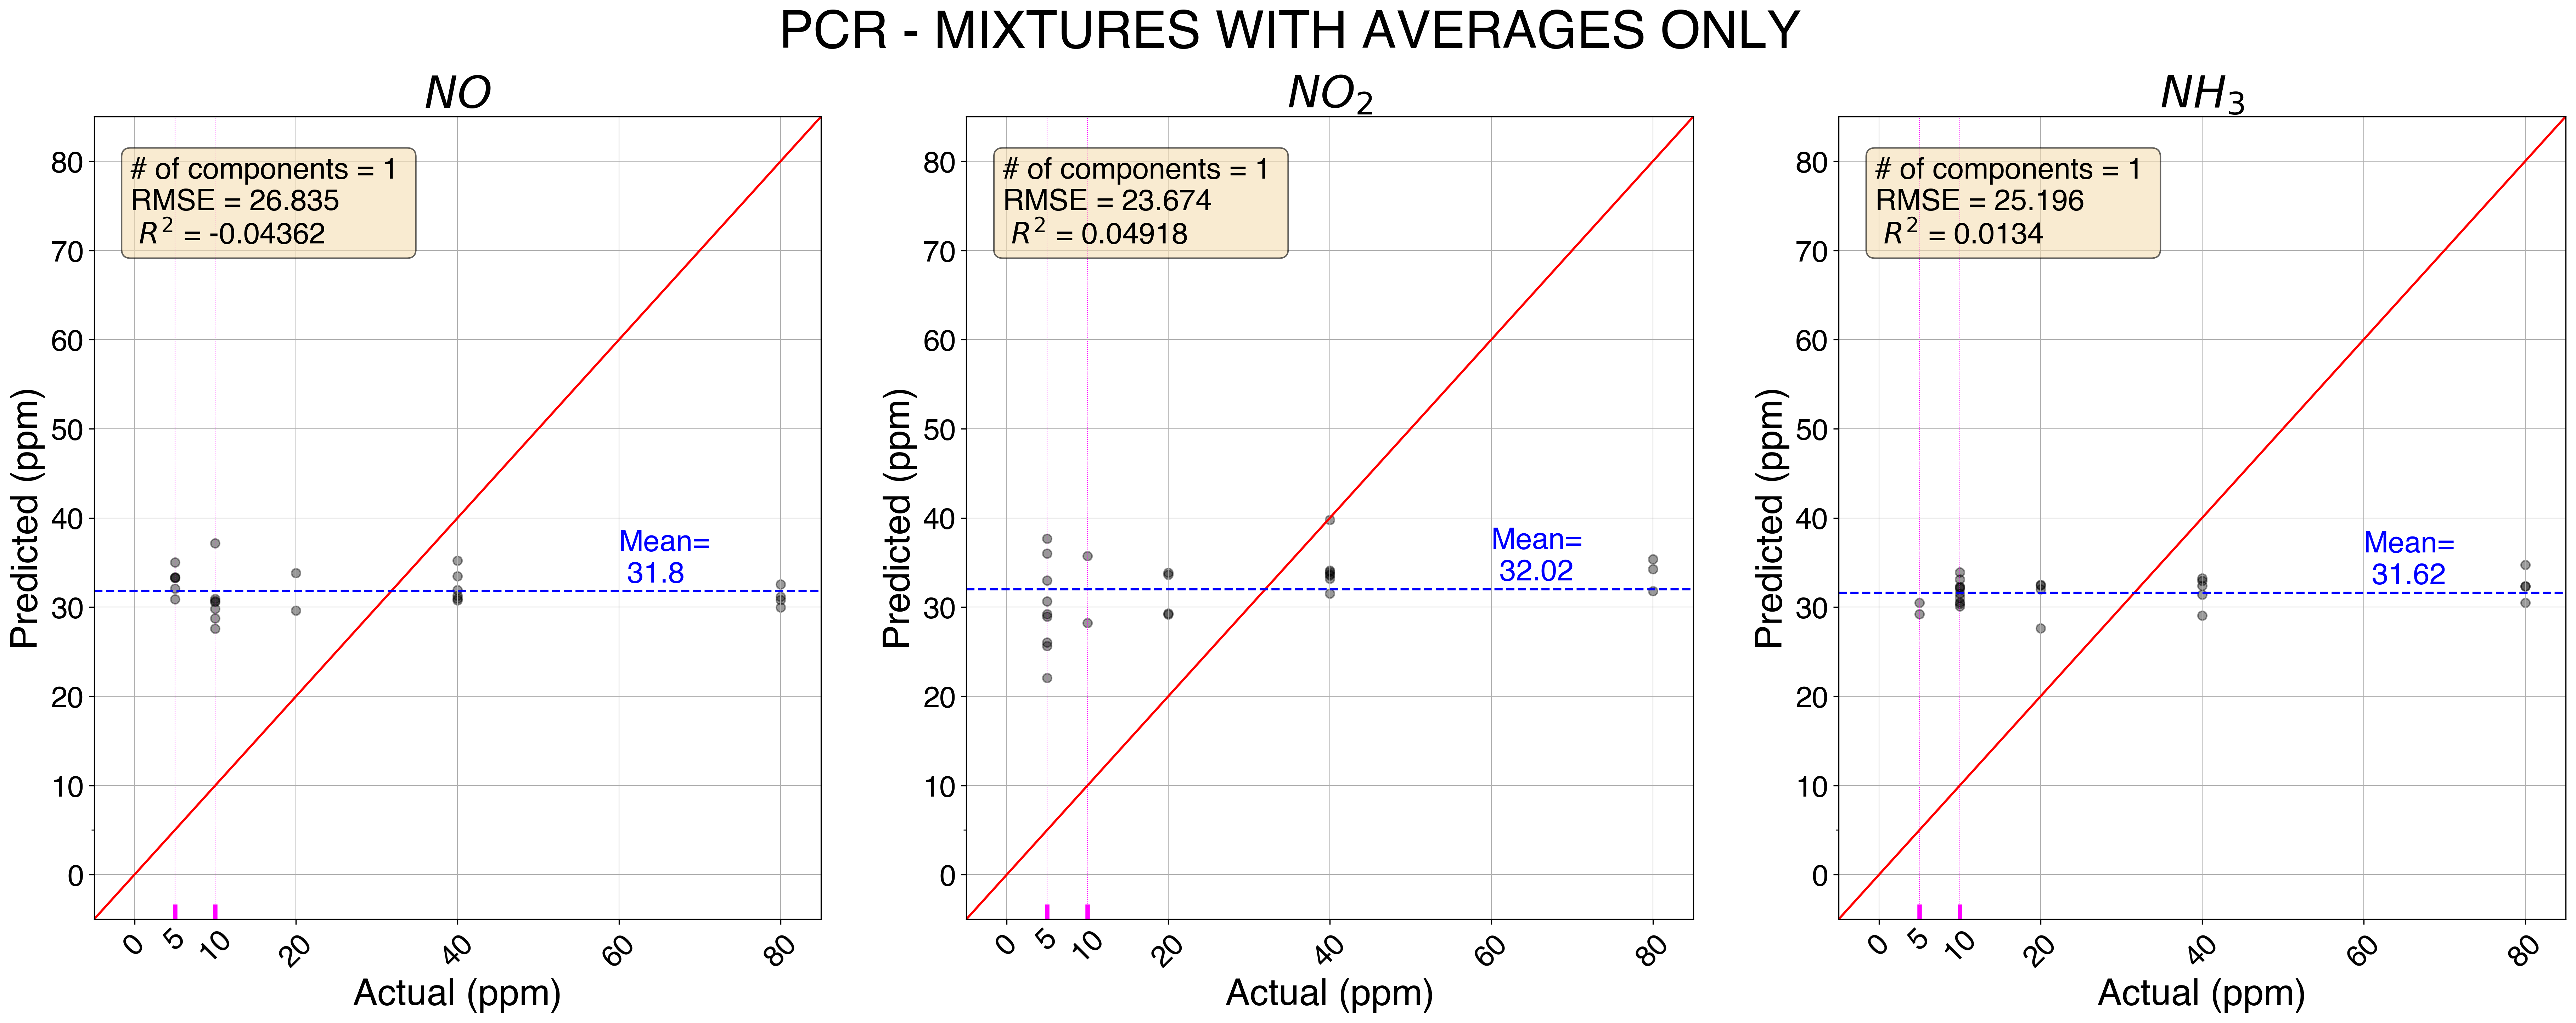
\includegraphics[width=0.8\textwidth, height = 3cm, keepaspectratio]{../../figures/pcr-act-vs-pred-avg-feat.png}
			\caption{Actual vs. pred for \textbf{mixtures}.}
			\label{fig:pcr-act-vs-pred-avg-feat}
		\end{figure}

\end{frame}

\begin{frame}
	\frametitle{Results}
	\framesubtitle{PLSR}
		
		\begin{figure}
			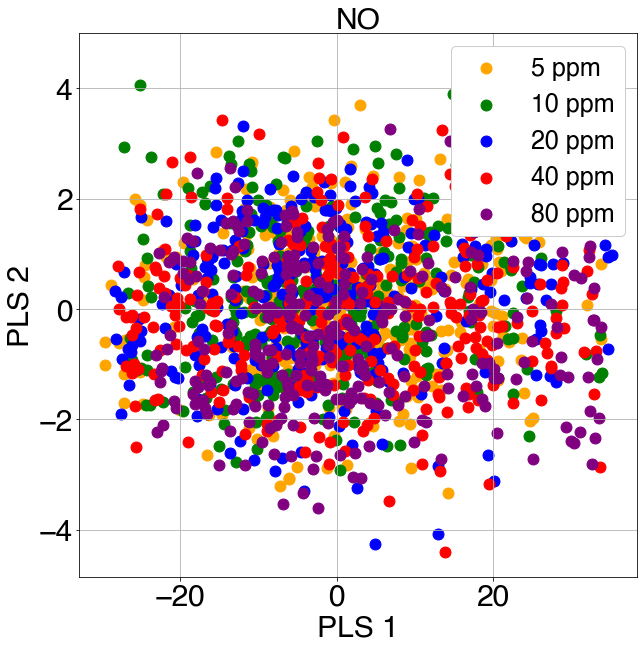
\includegraphics[width=0.30\textwidth]{../../figures/plsNO.png}
			\hfill
			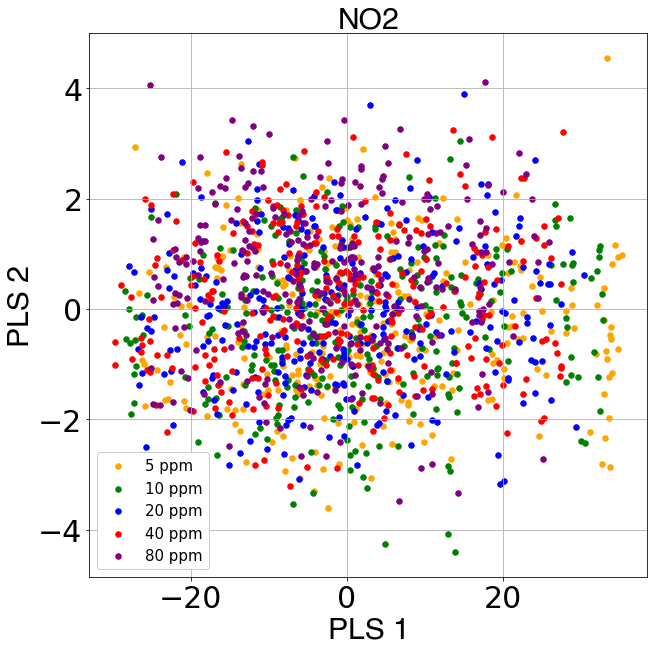
\includegraphics[width=0.30\textwidth]{../../figures/plsNO2.png}
			\hfill
			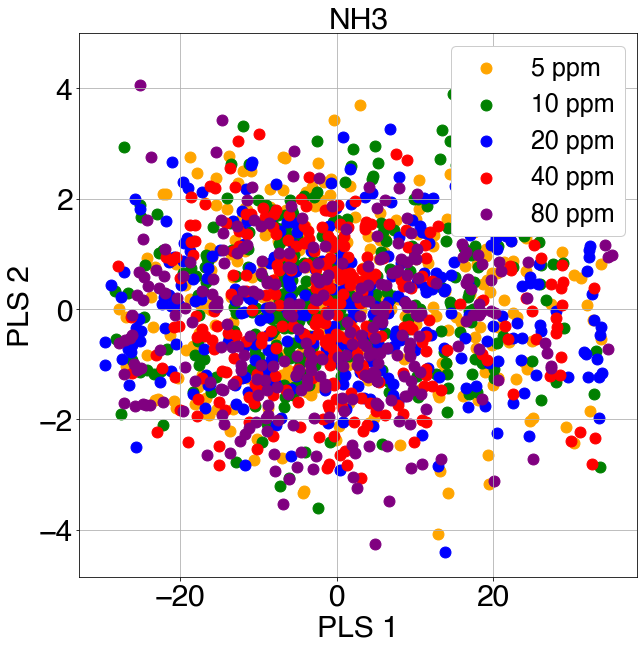
\includegraphics[width=0.30\textwidth]{../../figures/plsNH3.png}
			\caption{PLS scores for \textbf{exposures}.}
			\label{fig:pls}
		\end{figure}
		
		\begin{figure}
			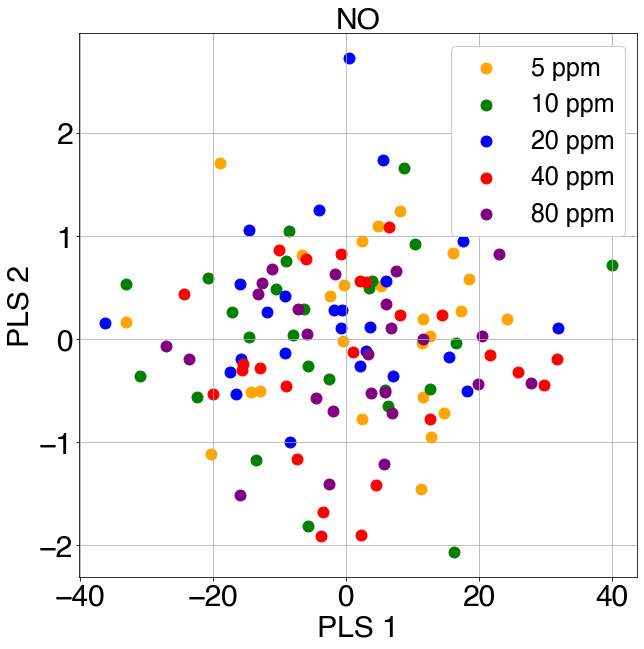
\includegraphics[width=0.30\textwidth, height = 3cm, keepaspectratio]{../../figures/plsNO-avg-feat.png}
			\hfill
			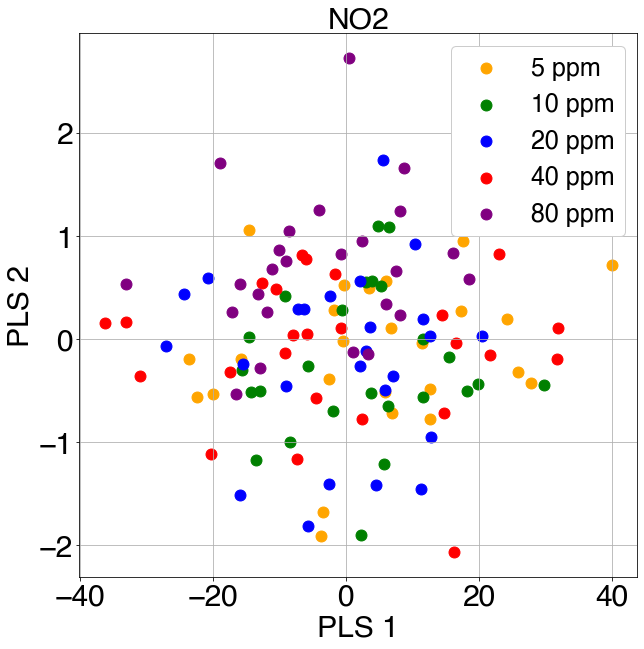
\includegraphics[width=0.30\textwidth, height = 3cm, keepaspectratio]{../../figures/plsNO2-avg-feat.png}
			\hfill
			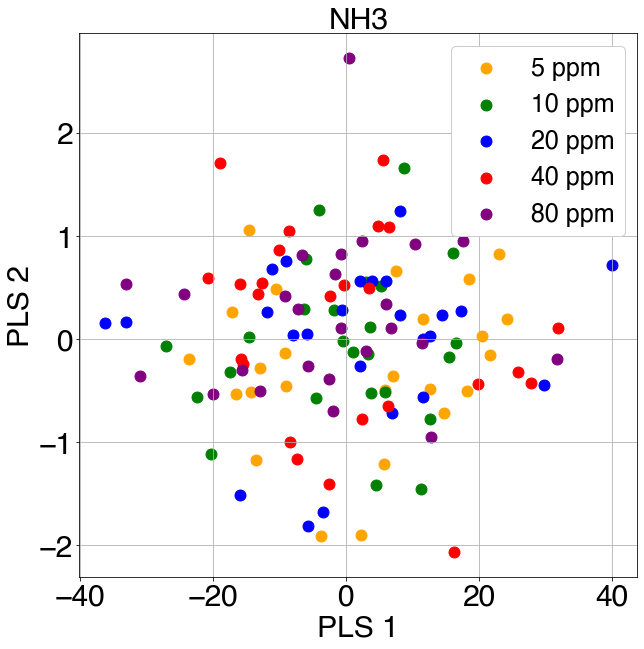
\includegraphics[width=0.30\textwidth, height = 3cm, keepaspectratio]{../../figures/plsNH3-avg-feat.png}
			\caption{PLS scores for \textbf{mixtures}.}
			\label{fig:pls-avg-only}
		\end{figure}
	
\end{frame}

\begin{frame}
	\frametitle{Results}
	\framesubtitle{PLSR}
		\begin{figure}
			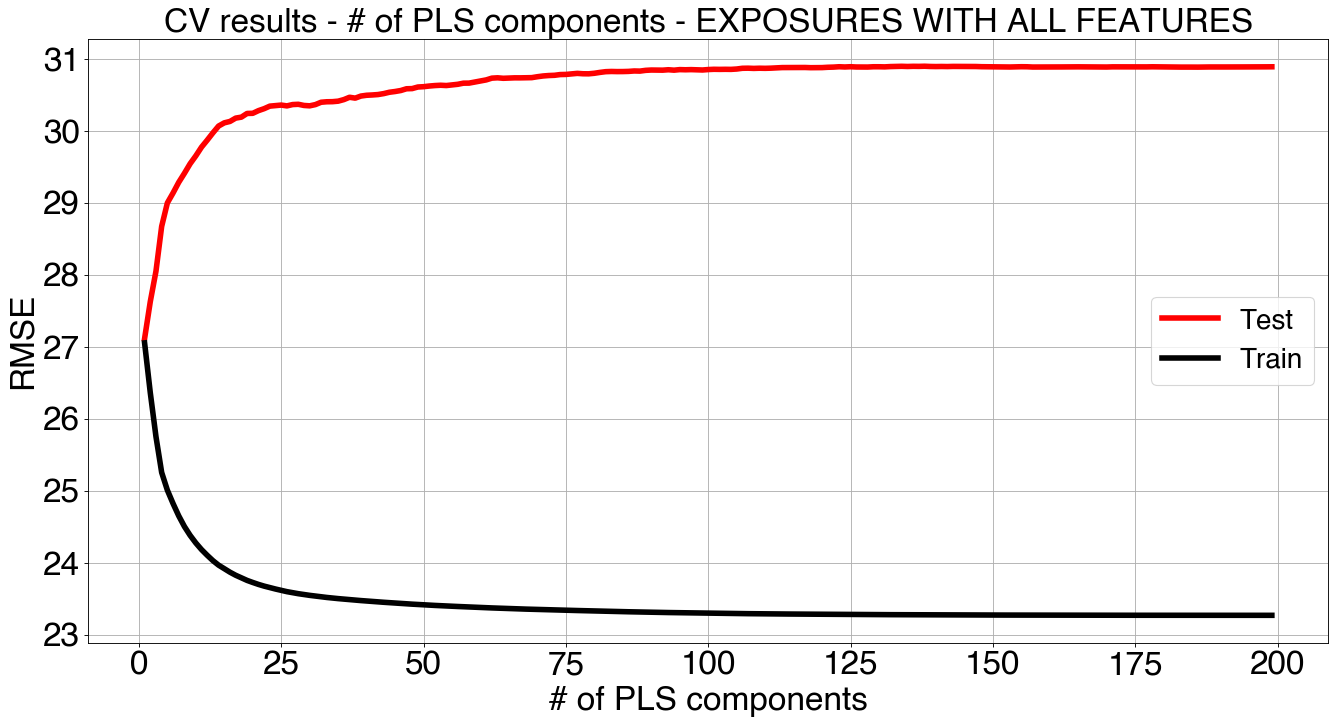
\includegraphics[width=0.5\linewidth]{../../figures/pls-cv.png}
			\caption{CV results for \textbf{exposures}.}
			\label{fig:pls-cv} 
		\end{figure}
		
		\begin{figure}
			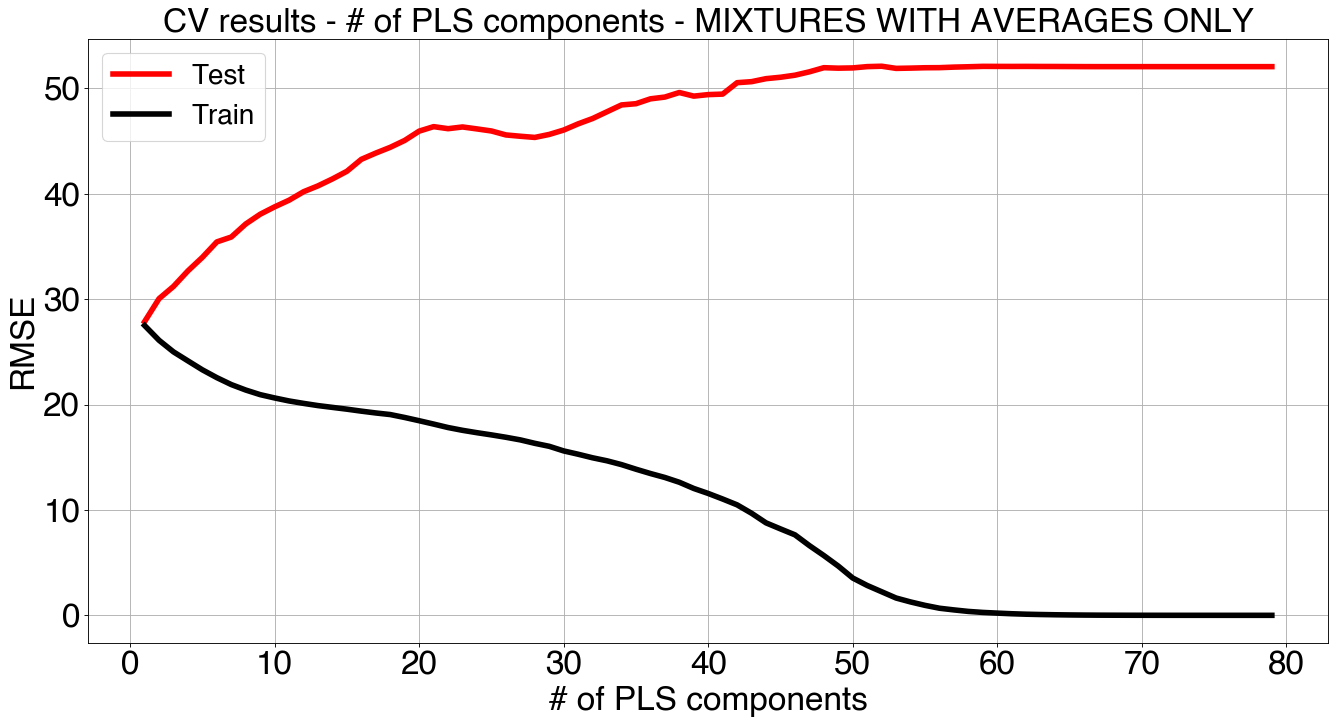
\includegraphics[width=0.5\linewidth]{../../figures/pls-cv-avg-feat.png}
			\caption{CV results for \textbf{mixtures}.}
			\label{fig:pls-cv-avg-feat}
		\end{figure}
\end{frame}

\begin{frame}
	\frametitle{Results}
	\framesubtitle{PLSR}
	
	\begin{figure}
		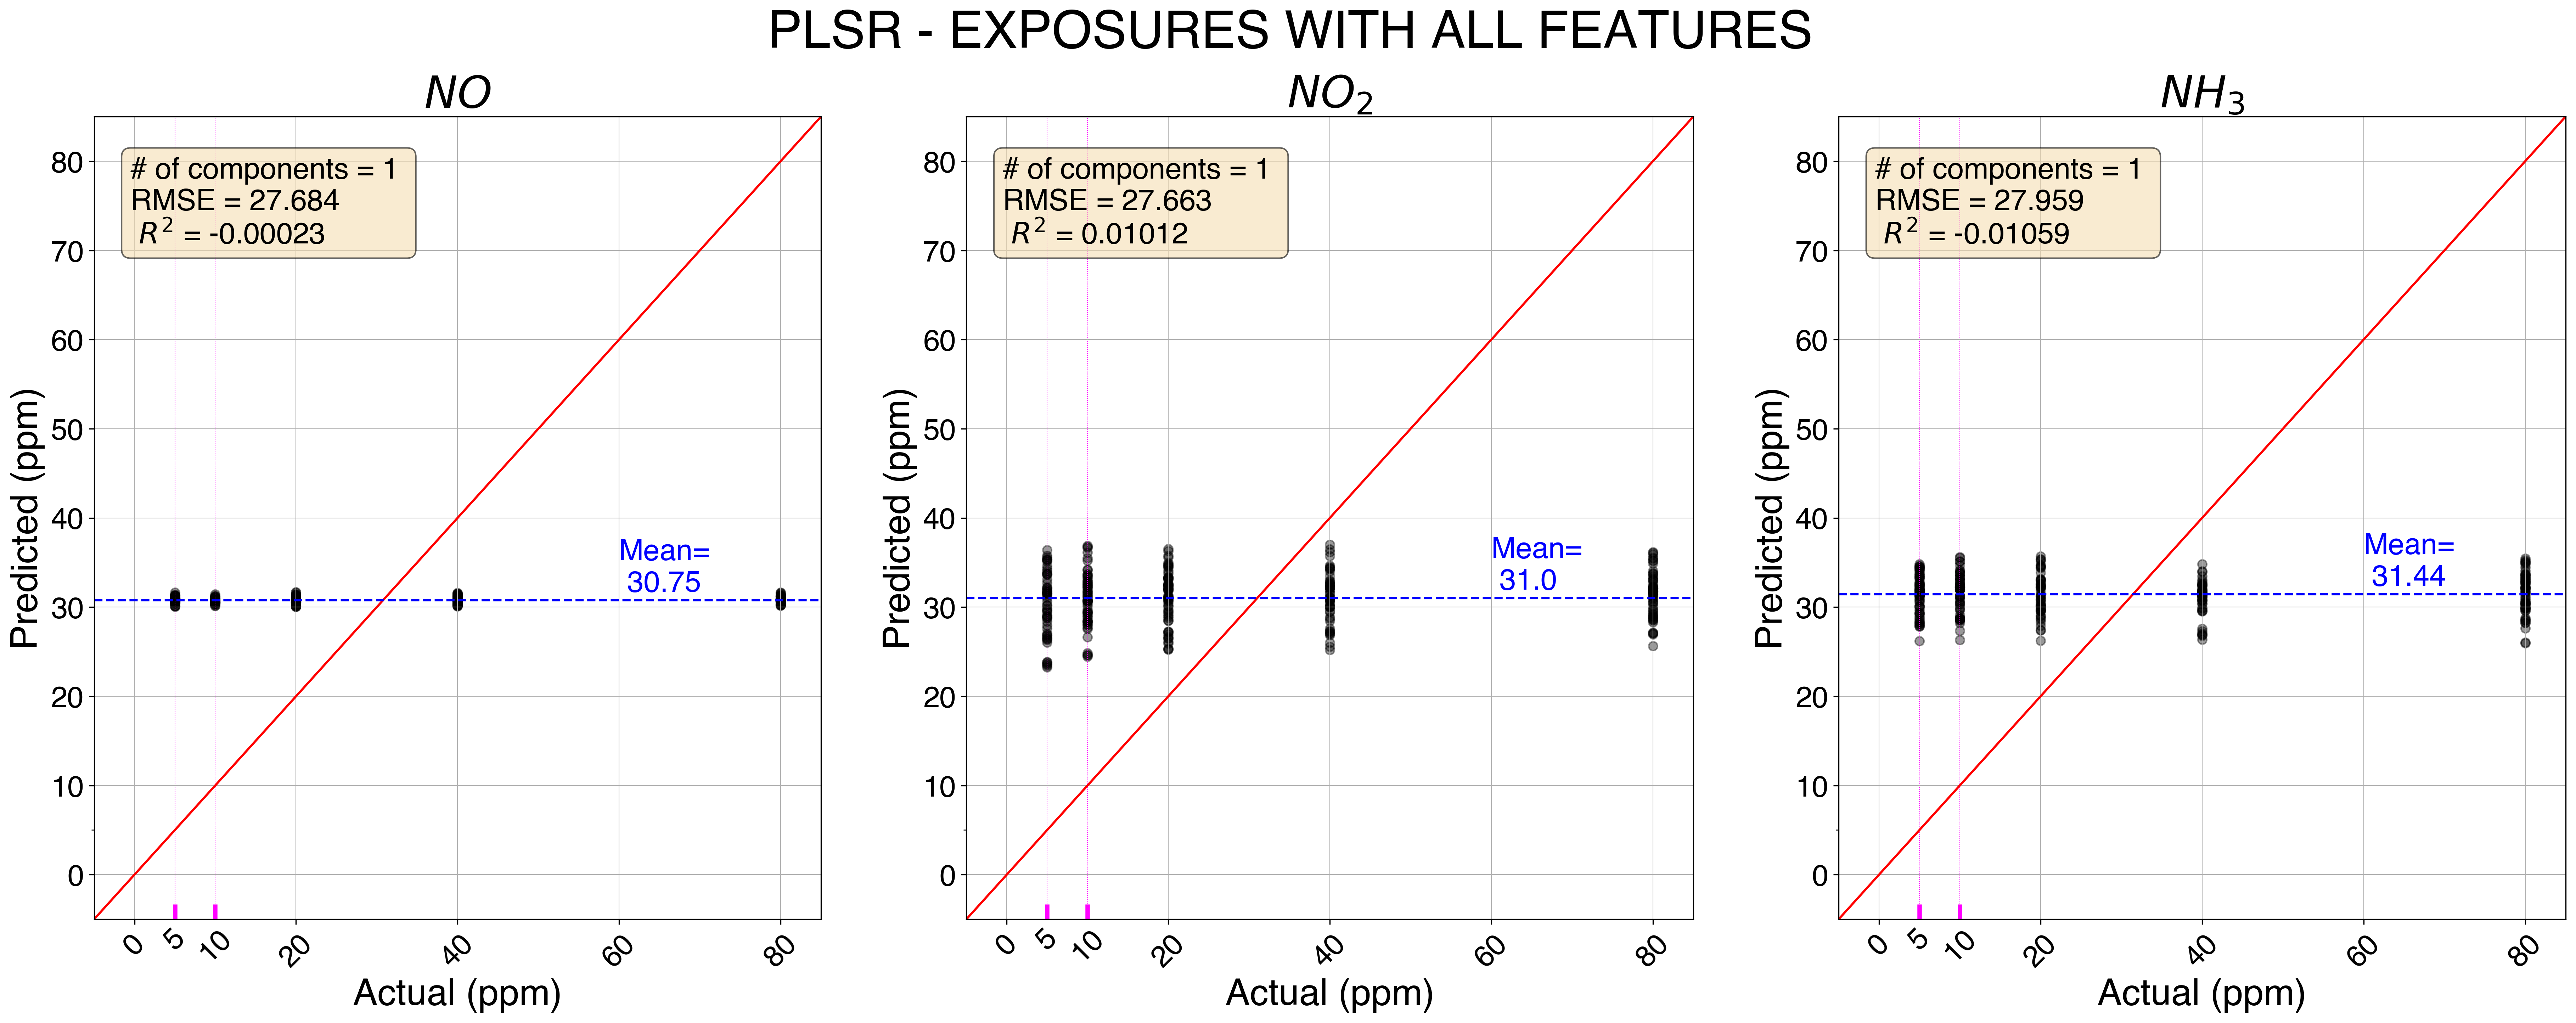
\includegraphics[width=0.8\textwidth, height = 3cm, keepaspectratio]{../../figures/plsr-act-vs-pred.png}
		\caption{Actual vs. pred for \textbf{exposures}.}
	\end{figure}
	
	\begin{figure}
		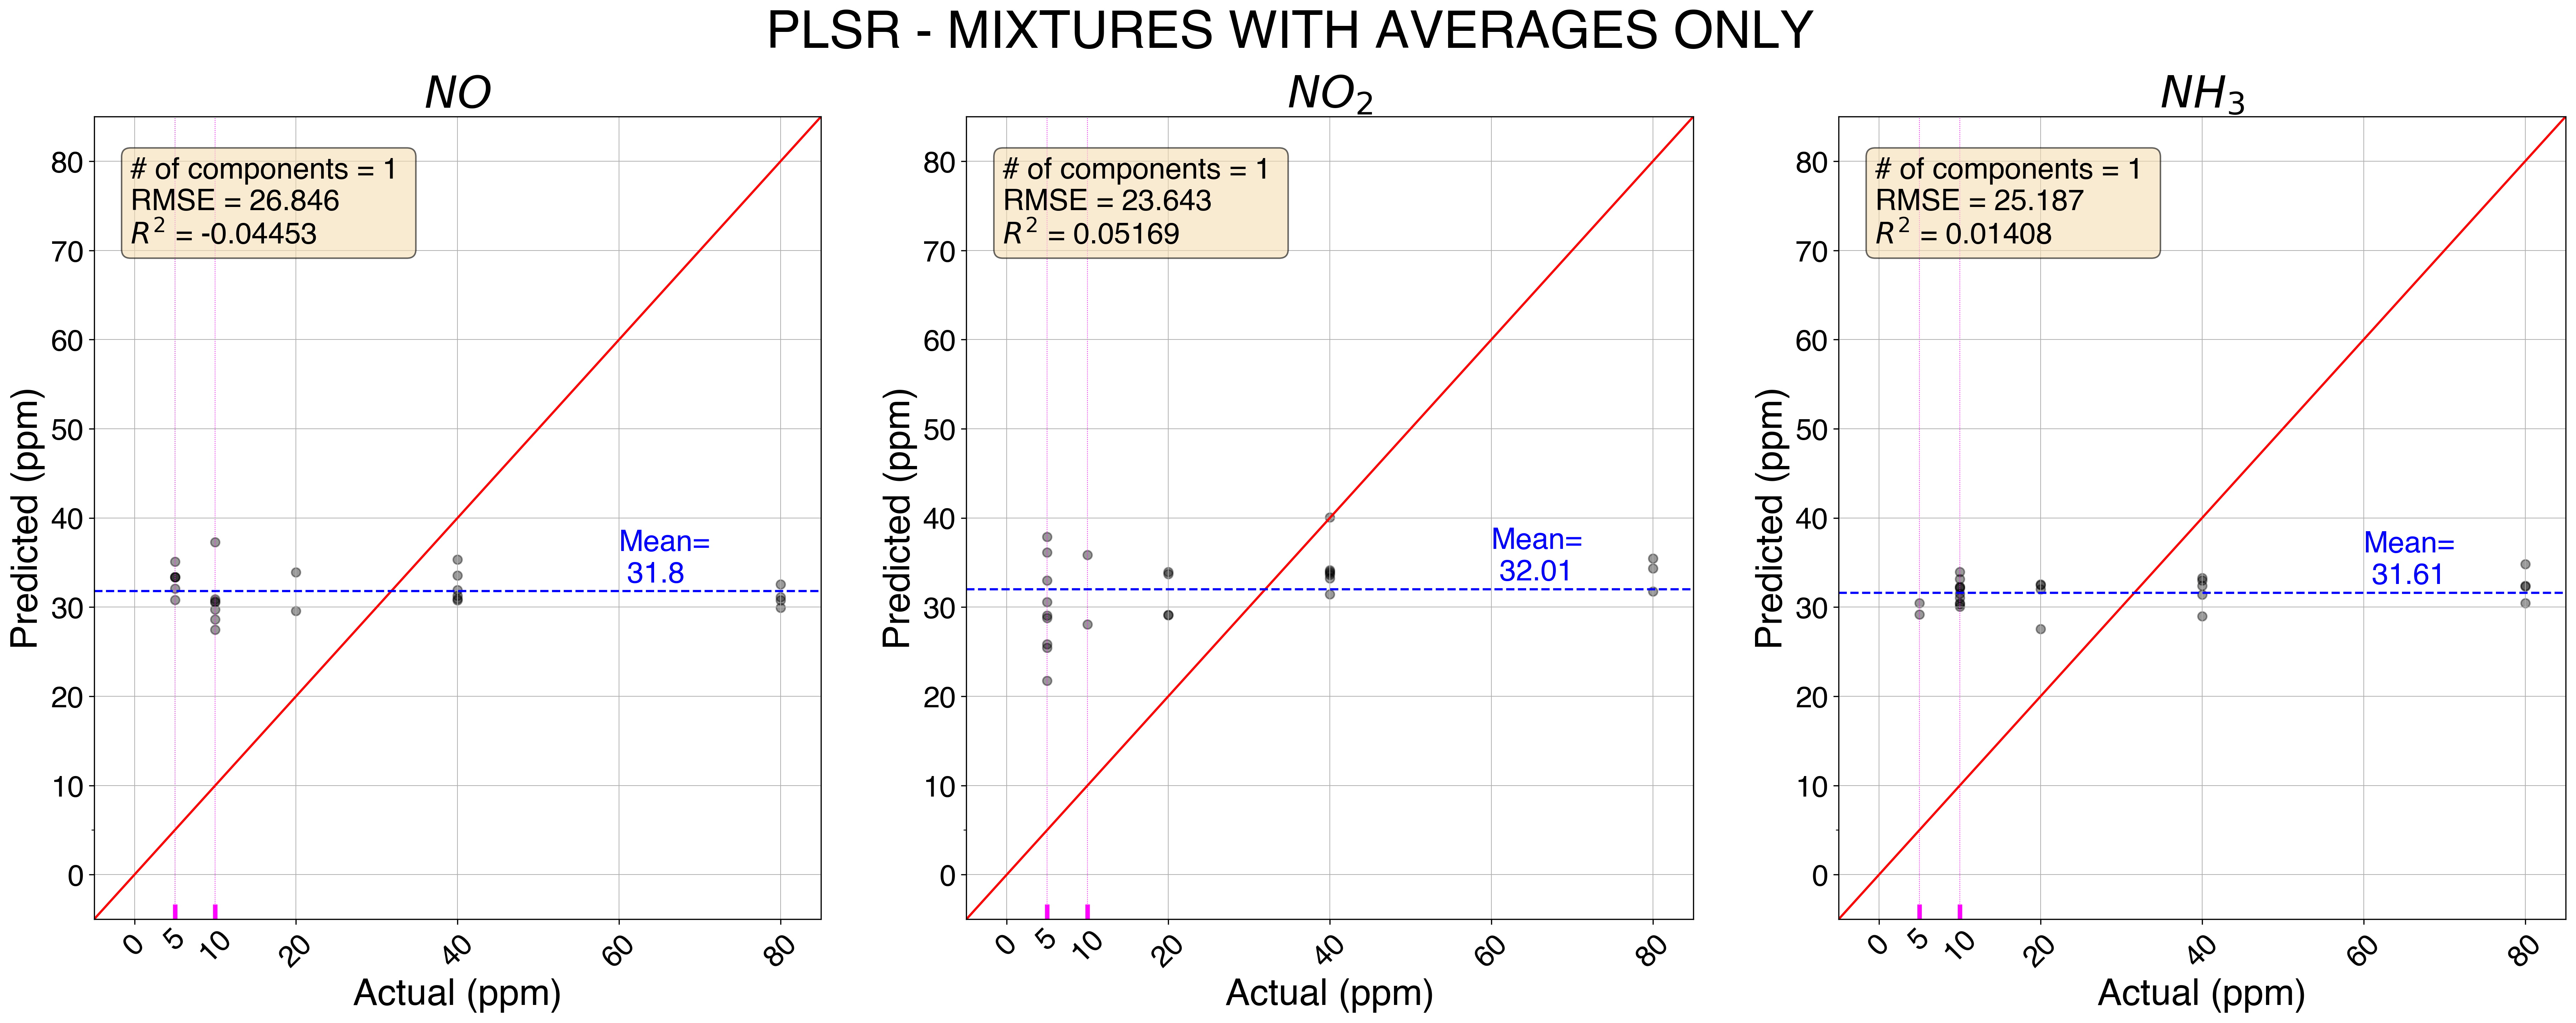
\includegraphics[width=0.8\textwidth, height = 3cm, keepaspectratio]{../../figures/plsr-act-vs-pred-avg-feat.png}
		\caption{Actual vs. pred for \textbf{mixtures}.}
	\end{figure}
	
\end{frame}

\begin{frame}
	\frametitle{Results}
	\framesubtitle{Ridge regression}
	
		\begin{figure}
		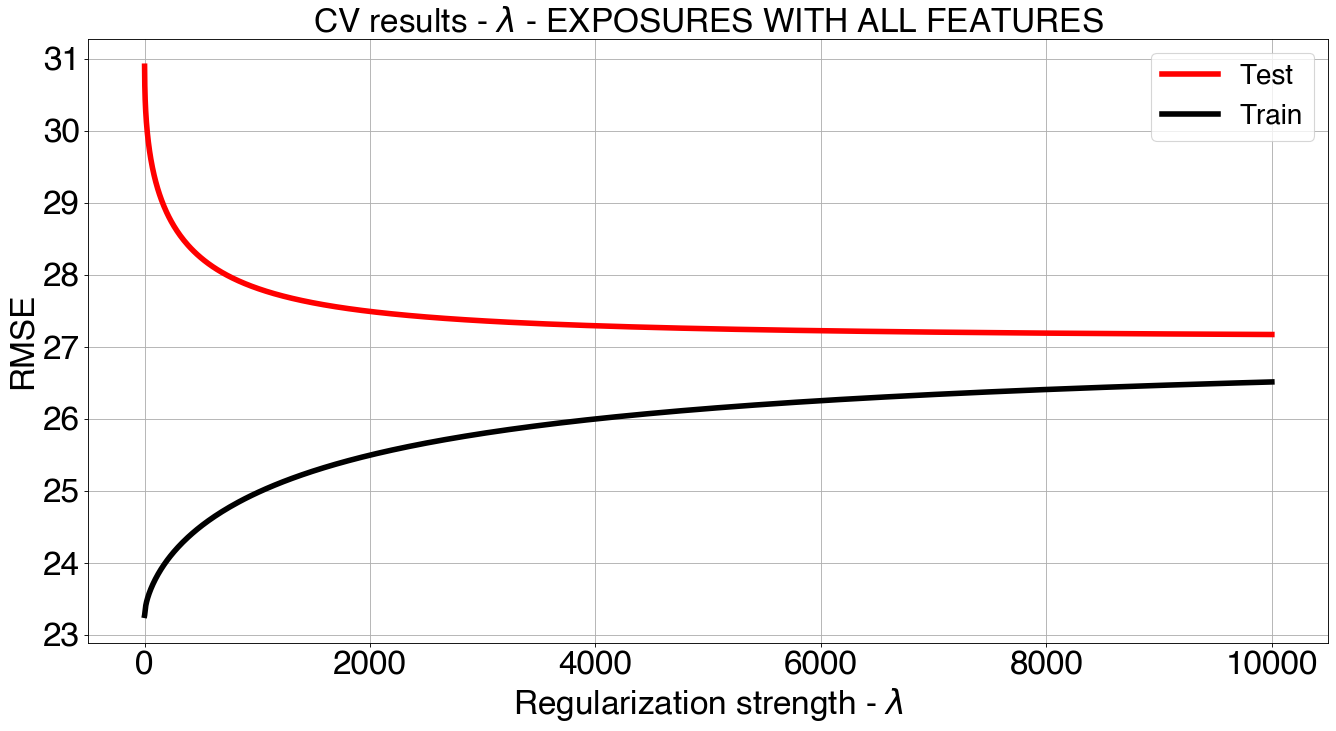
\includegraphics[width=0.5\linewidth]{../../figures/ridge-cv.png}
		\caption{CV results for \textbf{exposures}.}
	\end{figure}
	
	\begin{figure}
		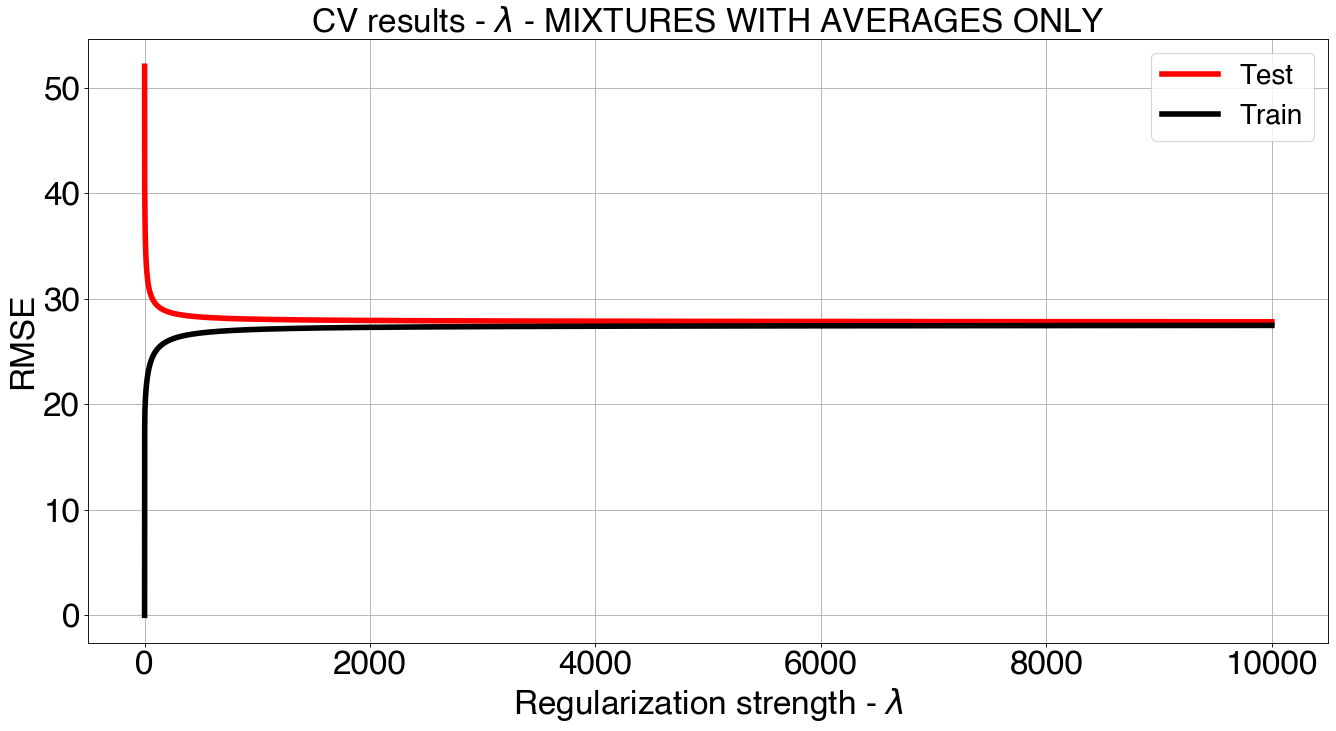
\includegraphics[width=0.5\linewidth]{../../figures/ridge-cv-avg-feat.png}
		\caption{CV results for \textbf{mixtures}.}
	\end{figure}
	
\end{frame}

\begin{frame}
	\frametitle{Results}
	\framesubtitle{Ridge regression}
	
		\begin{figure}
		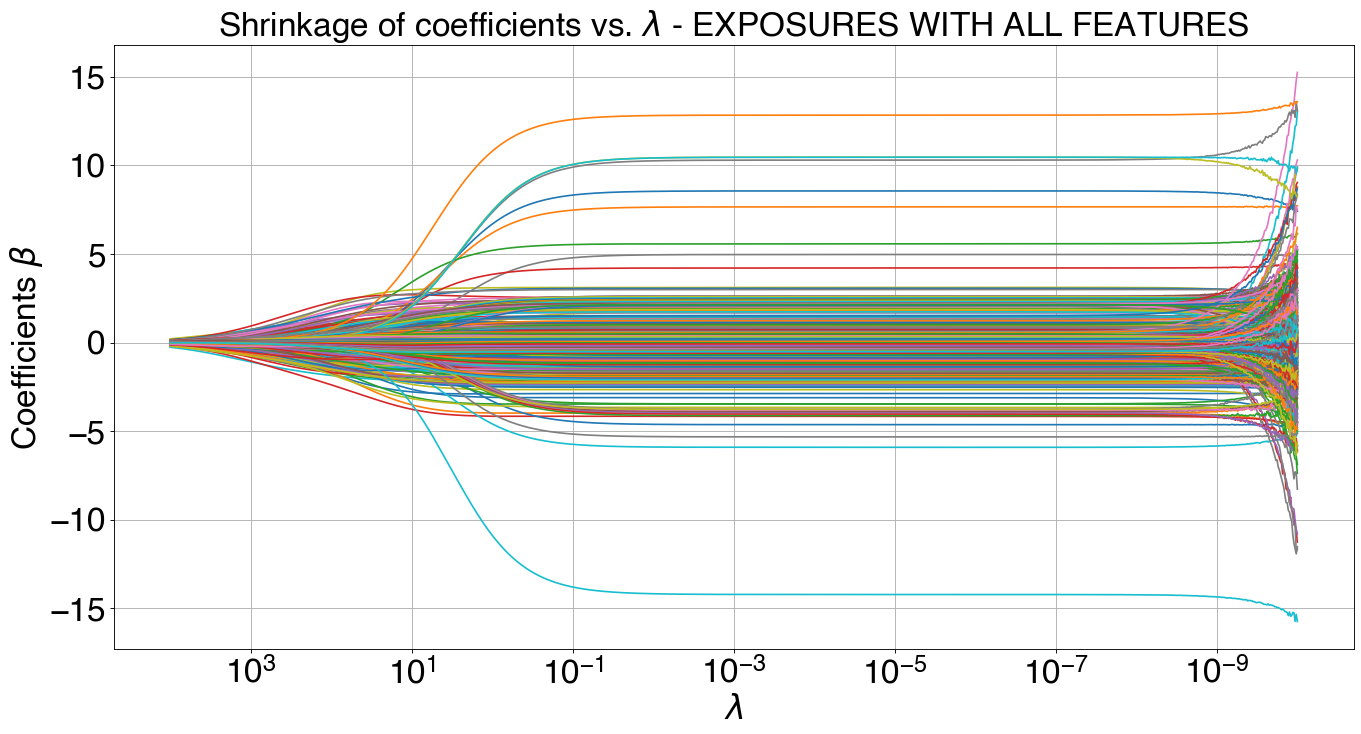
\includegraphics[width=0.5\linewidth]{../../figures/ridge-shrink.png}
		\caption{Shrinkage of coefficients for \textbf{exposures}.}
	\end{figure}
	
	\begin{figure}
		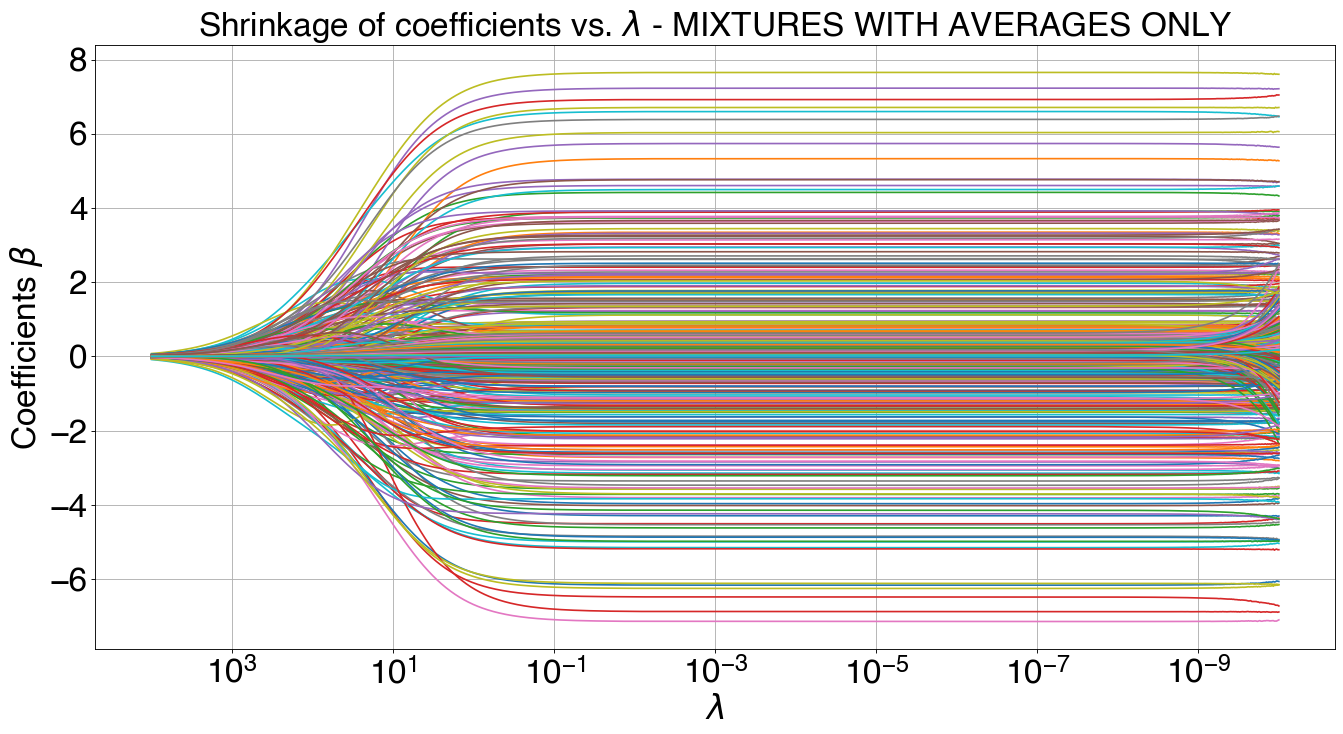
\includegraphics[width=0.5\linewidth]{../../figures/ridge-shrink-avg-feat.png}
		\caption{Shrinkage of coefficients for \textbf{mixtures}.}
	\end{figure}
	
\end{frame}

\begin{frame}
	\frametitle{Results}
	\framesubtitle{Ridge regression}
	
		\begin{figure}
		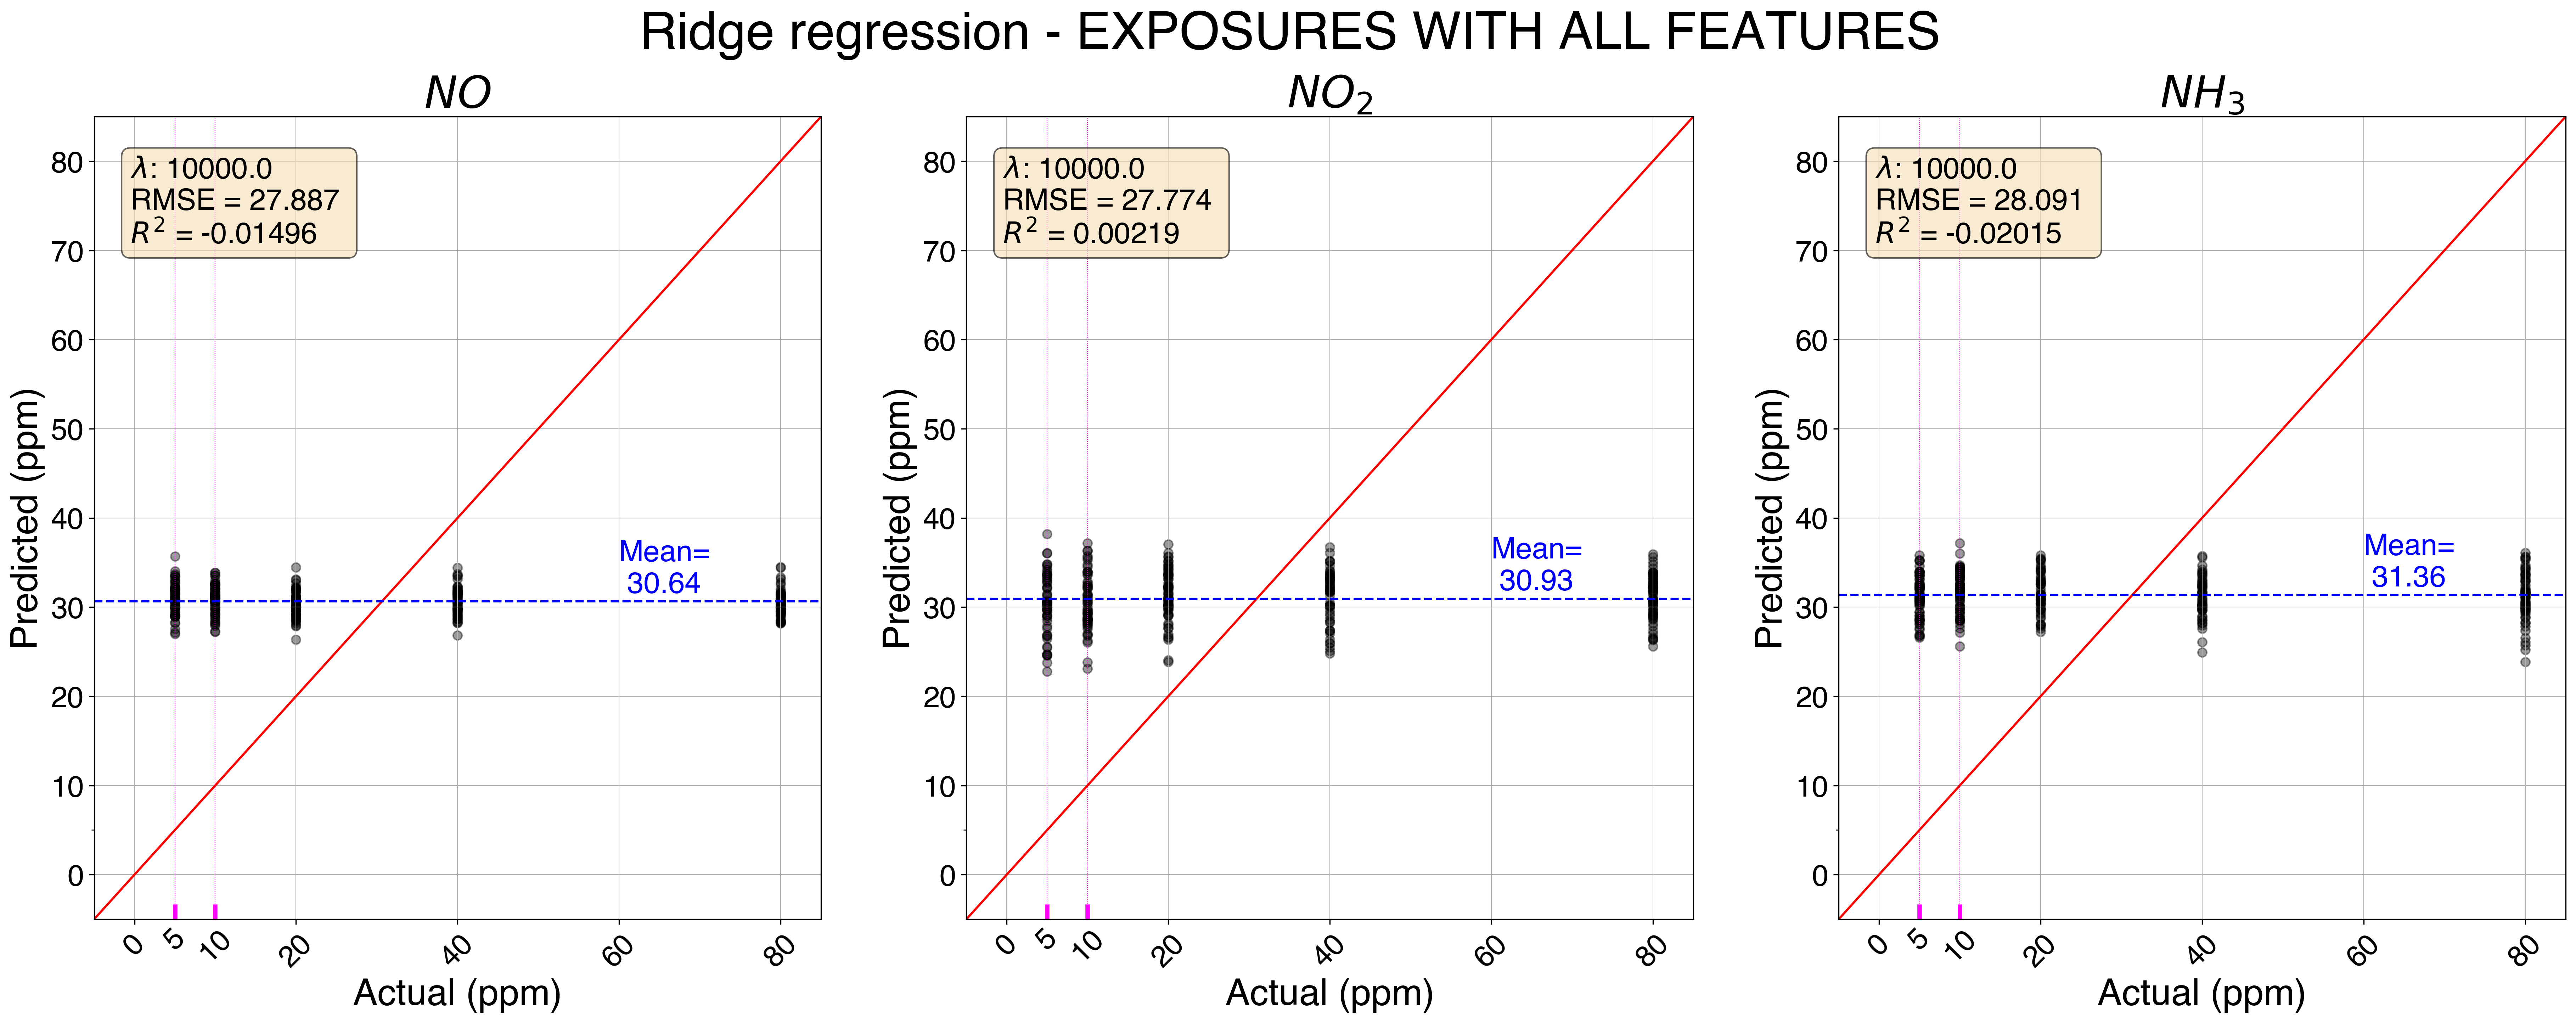
\includegraphics[width=0.8\textwidth, height = 3cm, keepaspectratio]{../../figures/ridge-act-vs-pred.png}
		\caption{Actual vs. pred for \textbf{exposures}.}
	\end{figure}
	
	\begin{figure}
		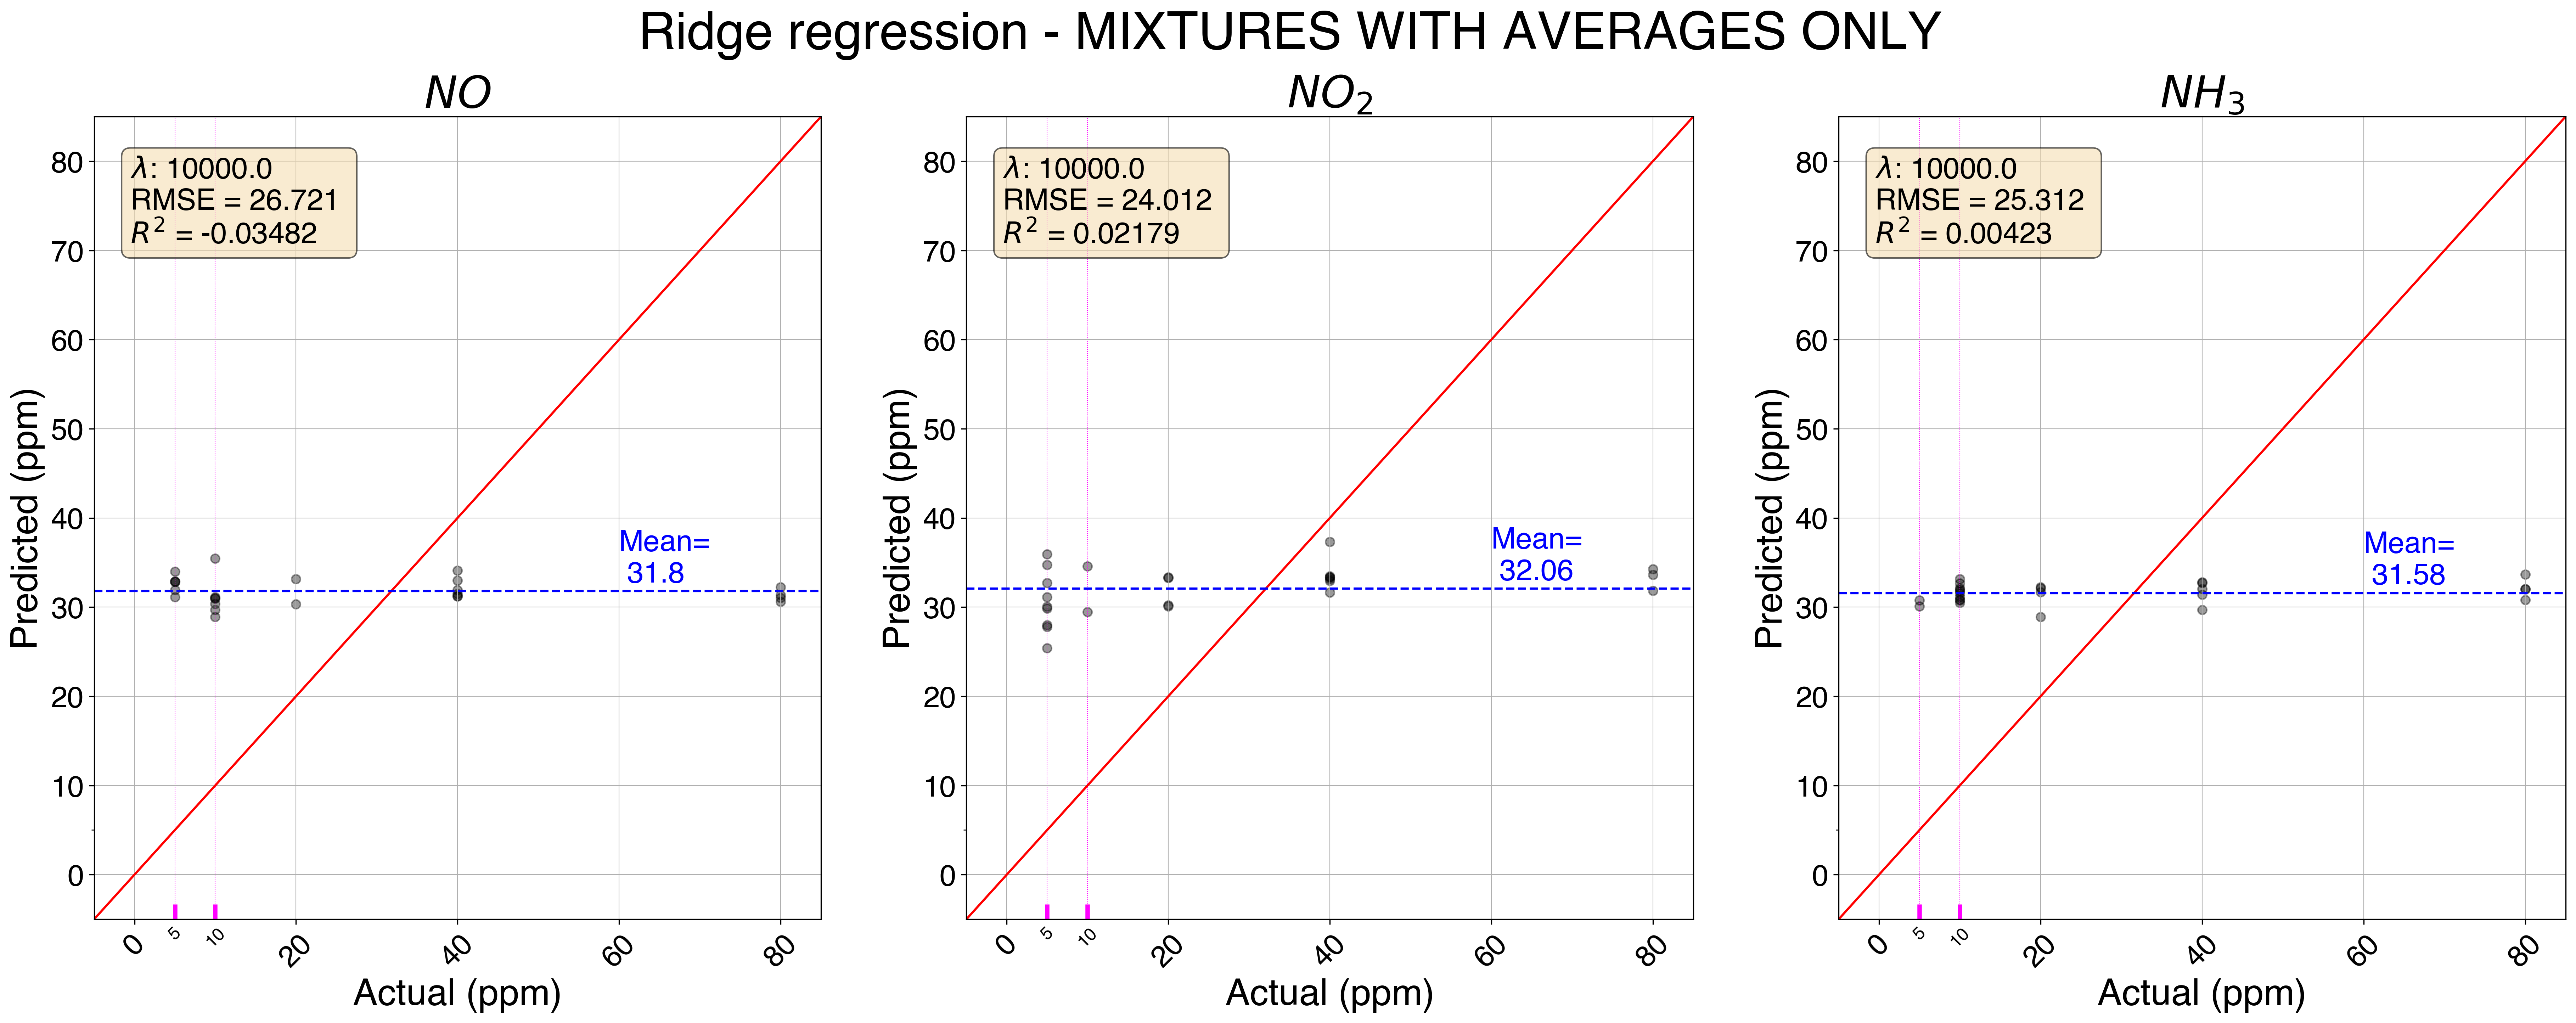
\includegraphics[width=0.8\textwidth, height = 3cm, keepaspectratio]{../../figures/ridge-act-vs-pred-avg-feat.png}
		\caption{Actual vs. pred for \textbf{mixtures}.}
	\end{figure}

\end{frame}


%%%%%%%%%%%%%%%%%%%%%%%%%%%%%%%%%%%%%%%%%%%%%%%%%%%%%%%%%%%%%%%%%%%%%%%%%%%%%%%%%%%%%%%%%%%%%%%%%%%%%%%%%%
\section{Discussion}
\begin{frame}
	\frametitle{Discussion}
	
	\begin{itemize}
		\pause
		\item All models fail on predicting gas concentrations.
		\pause
		\item Slopes are not informative.
		\pause
		\item Averages might be informative but there is no linear order in it.
		\pause
		\item Predictions are centered approximately  around the target mean $\bar{y} = 31$ ppm.
		\pause
		\item Results show that less complex, under-fitting models are preferred.
		
	\end{itemize} 	
	
\end{frame}


\begin{frame}
	\frametitle{Discussion}
	\framesubtitle{Attempts at finding order}
		\begin{figure}
			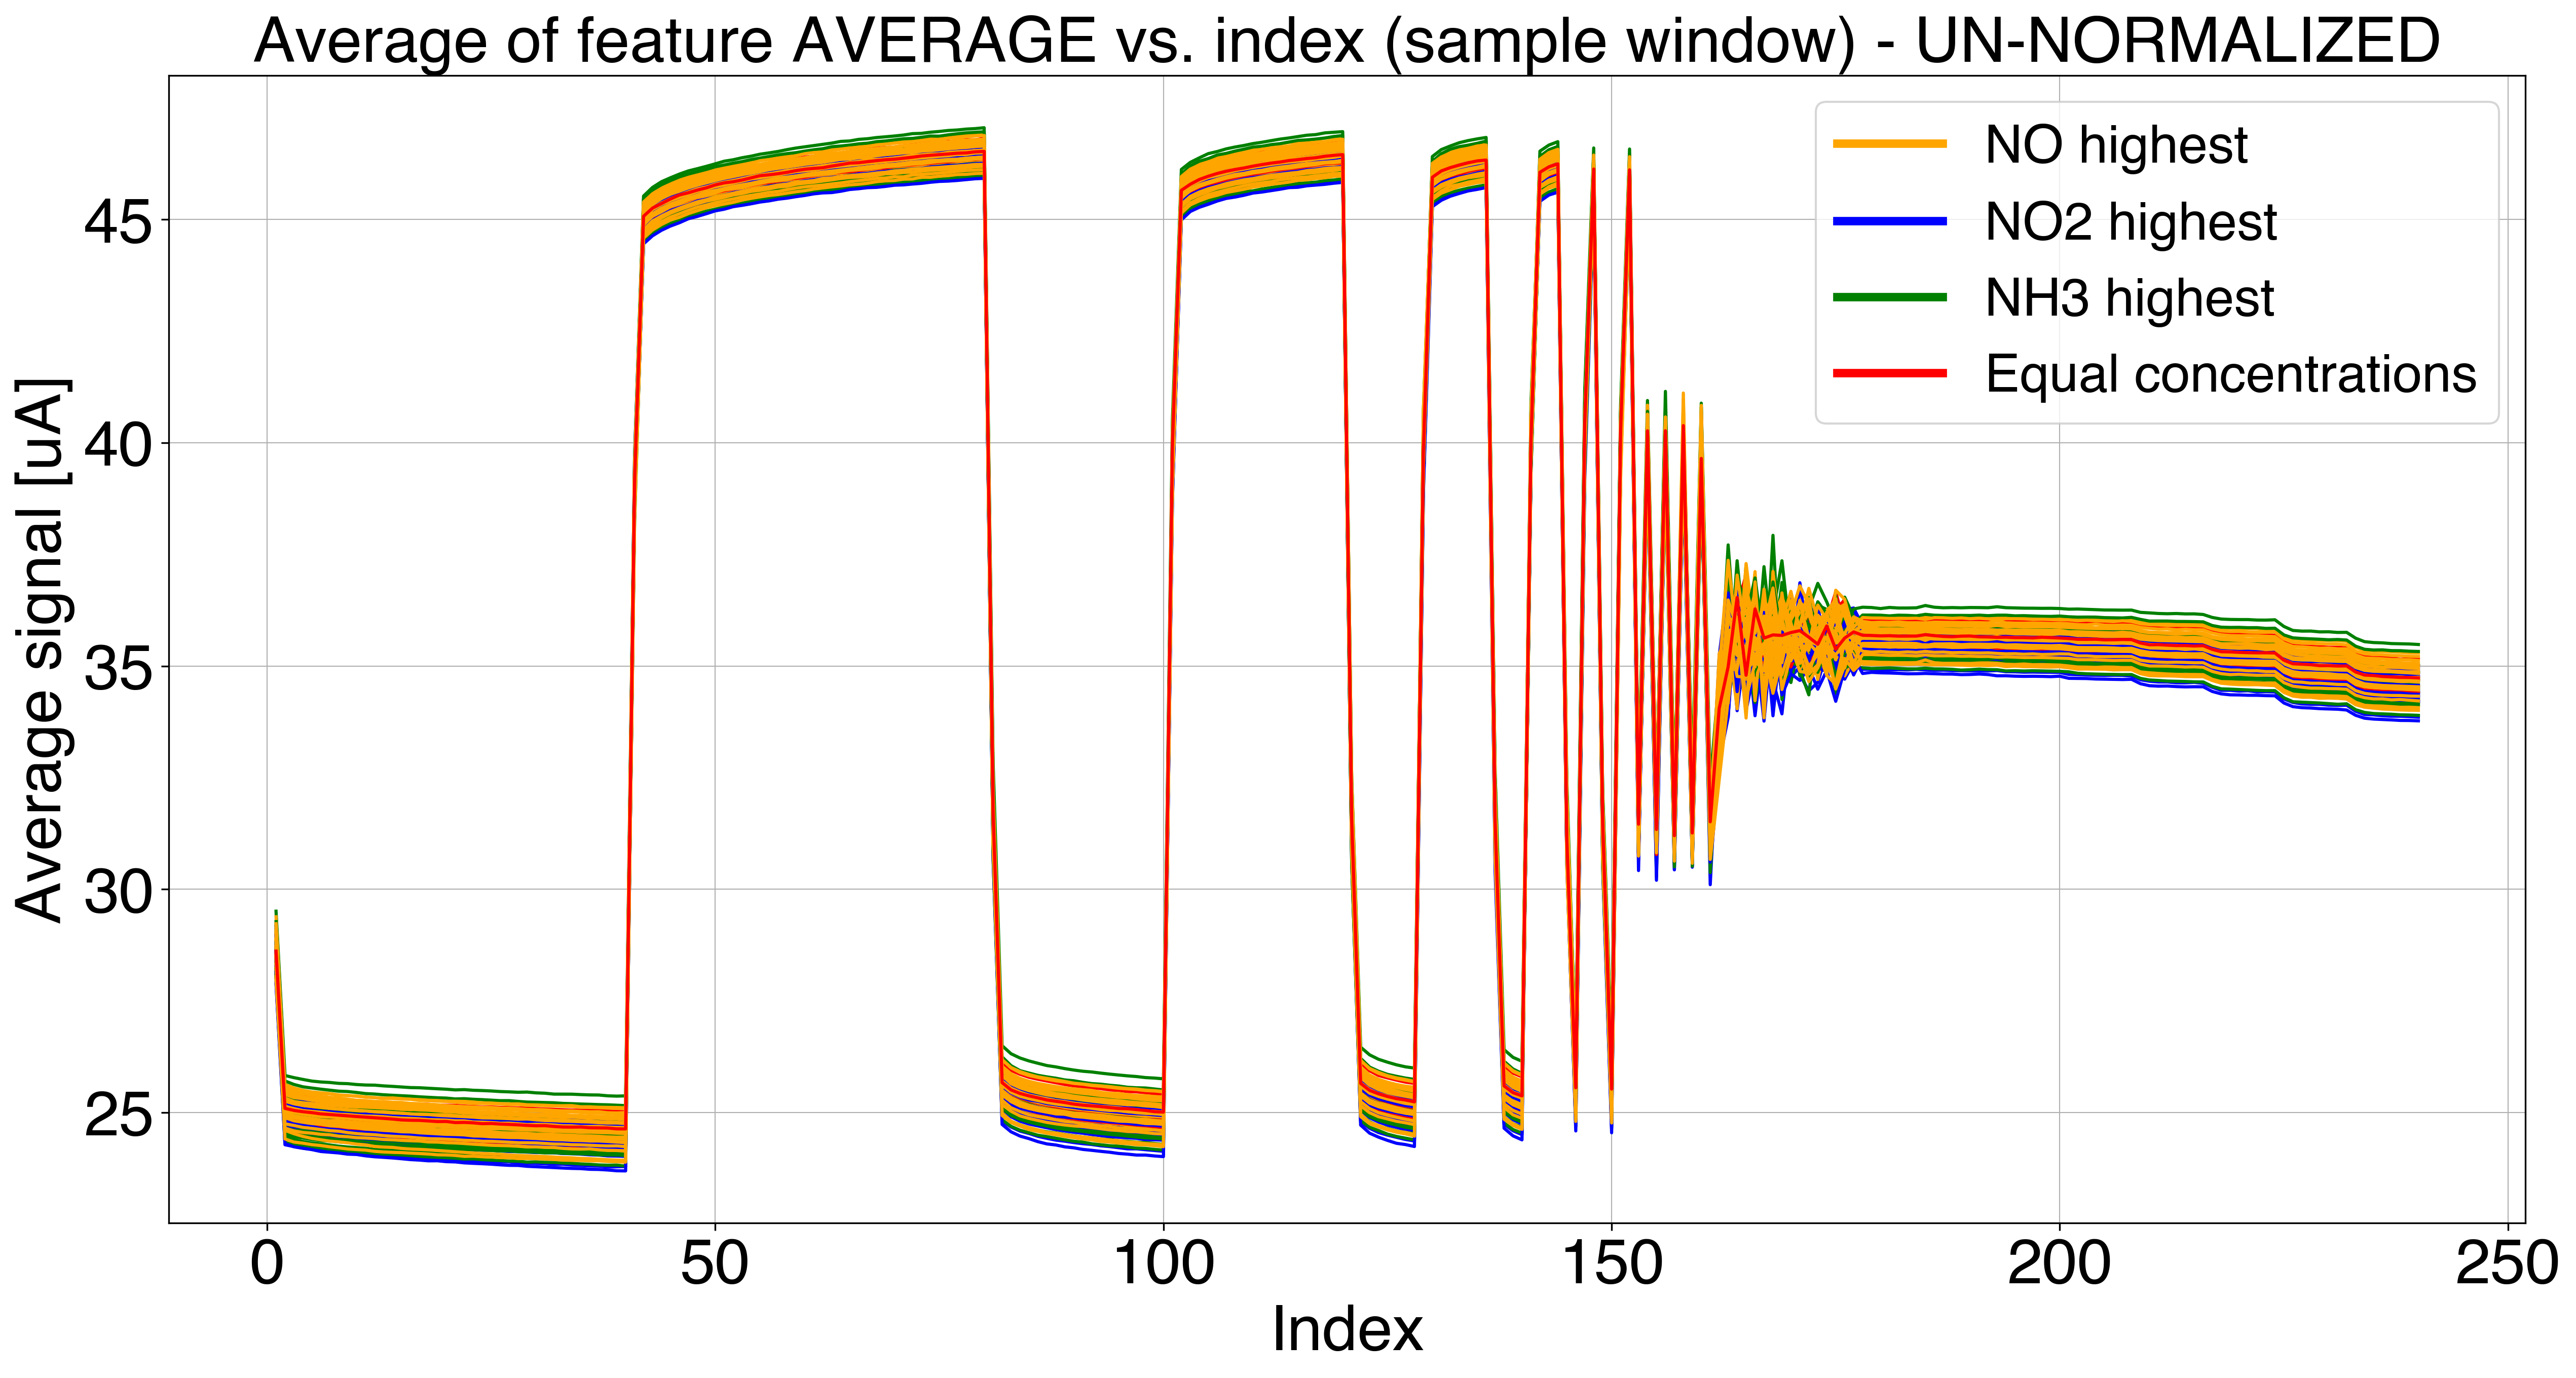
\includegraphics[width=1\linewidth]{../../figures/order1.png}
			\caption{Averaged sensor average divided by predominant gas. Each line corresponds to a unique \textbf{mixture}.}
		\end{figure}
\end{frame}

\begin{frame}
	\frametitle{Discussion}
	\framesubtitle{Attempts at finding order}
	
		\begin{figure}
		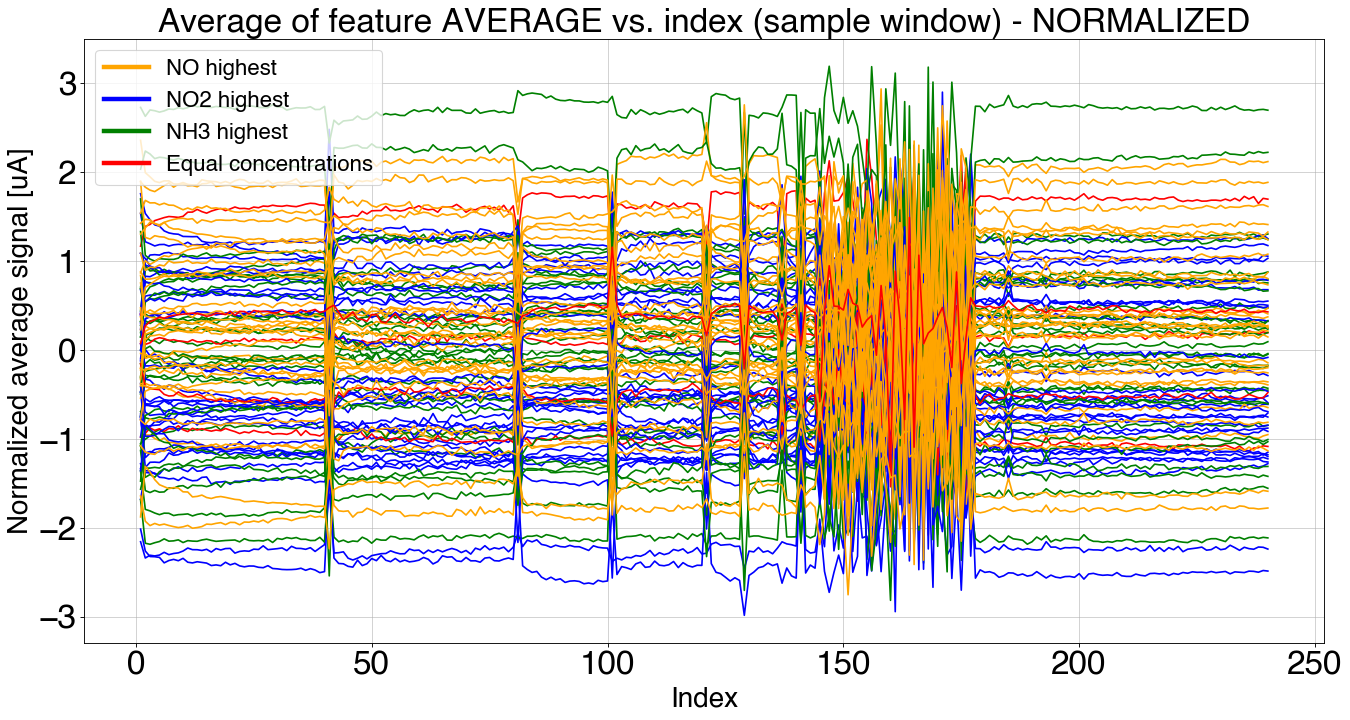
\includegraphics[width=1\linewidth]{../../figures/order1-norm.png}
		\caption{Normalized averaged sensor average divided by predominant gas. Each line corresponds to a unique \textbf{mixture}.}
	\end{figure}
\end{frame}

\begin{frame}
	\frametitle{Discussion}
	\framesubtitle{Attempts at finding order}
	\begin{figure}
	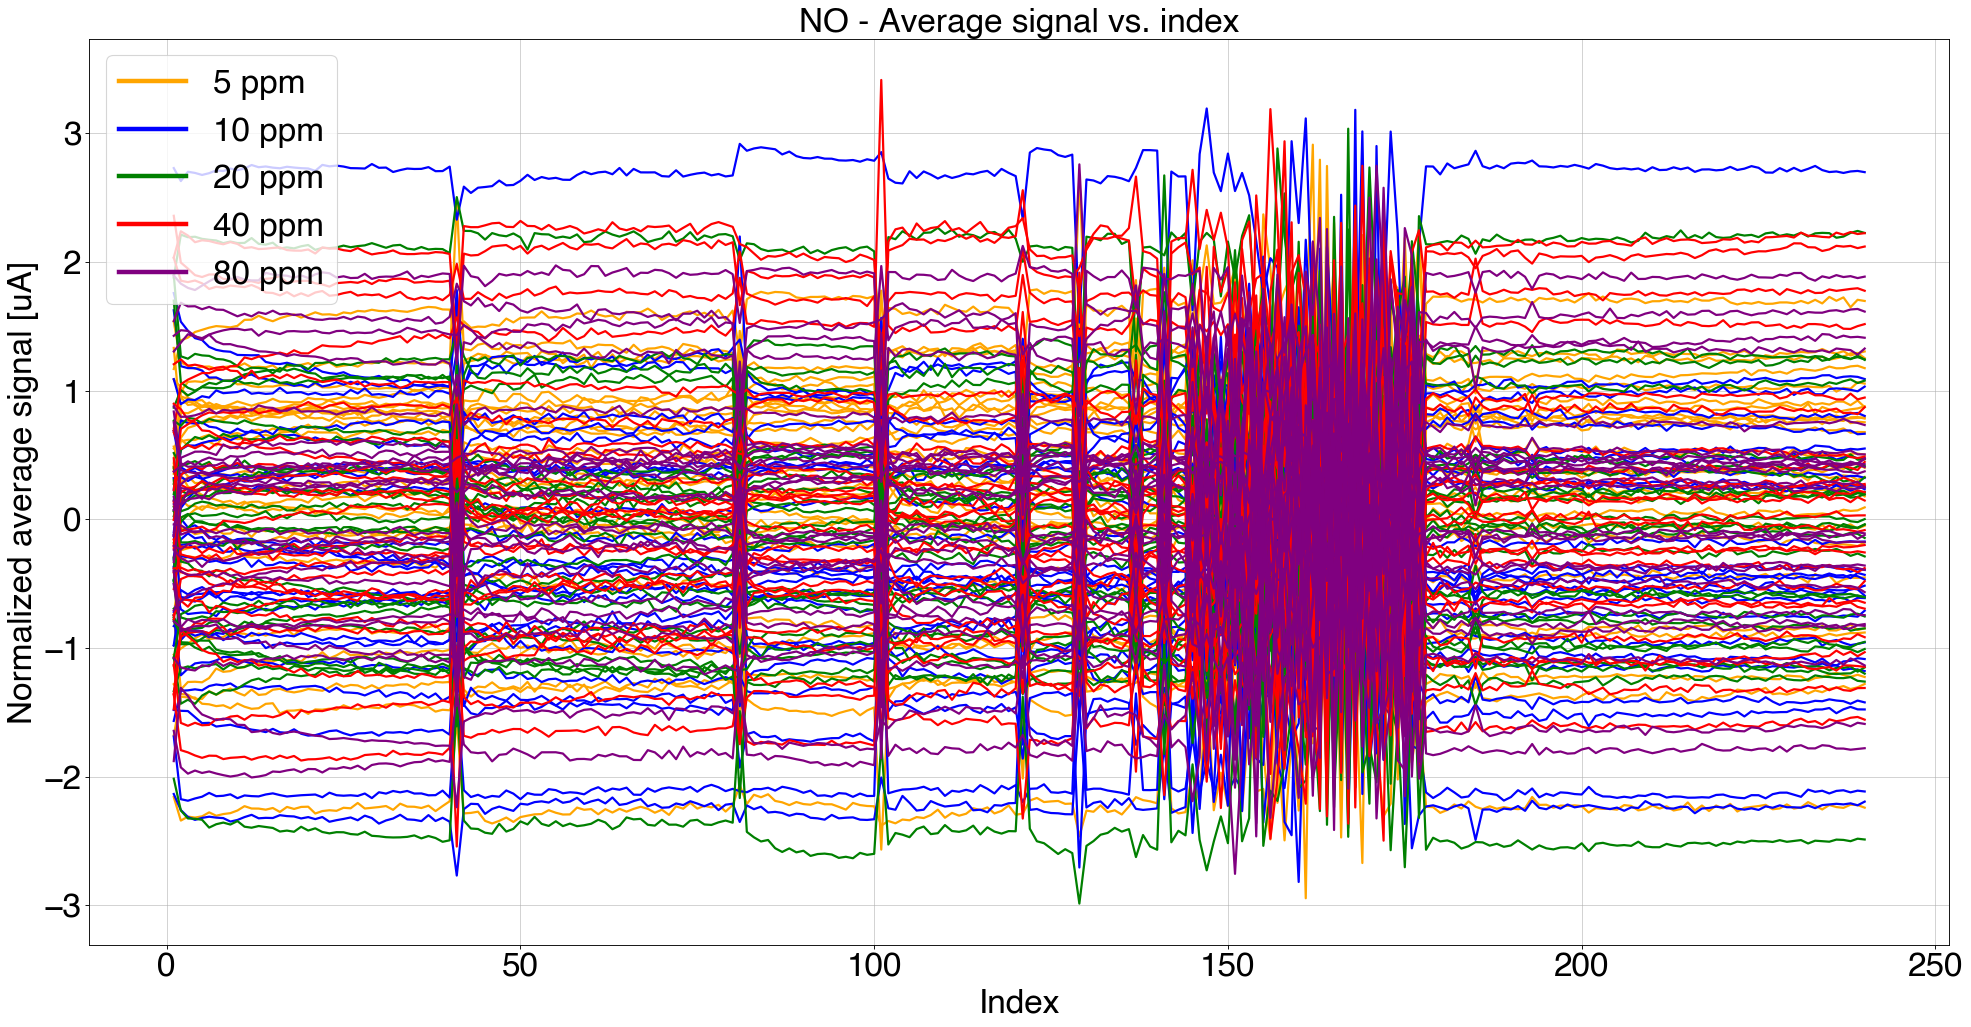
\includegraphics[width=1\linewidth]{../../figures/order2NO.png}
	\caption{Normalized sensor averaged for \ch{NO}. Each line corresponds to a unique \textbf{mixture}. The levels are the \ch{NO} concentrations of the mixture.}
\end{figure}
\end{frame}

%%%%%%%%%%%%%%%%%%%%%%%%%%%%%%%%%%%%%%%%%%%%%%%%%%%%%%%%%%%%%%%%%%%%%%%%%%%%%%%%%%%%%%%%%%%%%%%%%%%%%%%%%%
\section{Conclusion and Future work}
\begin{frame}
	\frametitle{Conclusion}
	\framesubtitle{and future work}
	
	\begin{enumerate}
		\pause
		\item Can frequency modulation be used to simultaneously quantify \nox and Ammonia concentrations?
		\begin{itemize}
			\pause
			\item \textbf{Possibly not.}
			\pause
			\item To answer this conclusively, different approaches need to be experimented with:
			\begin{enumerate}
				\pause
				\item Different shape-defining features? E.g. differences.
				\pause
				\item Different wave shape? E.g. Triangular waves.
				\pause
				\item Different models? E.g. Non-parametric models.
				\pause
				\item Different measurement window? e.g. lower sampling rate				
				\end{enumerate}
			\end{itemize}
	
		\pause
		\item Does the quality-of-fit vary over different prediction models?
		\begin{itemize}
			\pause
			\item \textbf{No.}
			\pause
			\item No point in selecting which model is "less bad".
		\end{itemize}
	\end{enumerate}

\pause
However, this work succeeded in pointing what does \textit{not} work. Arguably, this \textit{is as important as} know what works.

\end{frame}

\begin{frame}
	\frametitle{Master thesis}
	\framesubtitle{Defense seminar}
	\centering
	\Huge Thank you!
\end{frame}

\end{document}

